\documentclass[]{report}
\usepackage[margin=1in]{geometry}
\usepackage{url}
\usepackage{mathtools}
\usepackage{graphicx}
\usepackage{lscape}
\usepackage{listings}

\begin{document}
\linespread{1.3}

\title{Giving Up Smoking: Modelling how Social Networks Impact upon the Breaking of Habits}
\author{Matthew Smith (ID: 1003843) \\ Supervisor: Nathan Griffiths}
\date{\today}
\maketitle
\begin{abstract}
This project provides a proof-of-concept agent-based model for the problem of how social networking impacts on the behaviour of smoking cessation. By attempting to build a basic model of human smoking behaviours and defining interactions, this model allows for  simulations using, in theory, any number of autonomous entities. Through simulations, it appears that the quantity and social location of humans in networks significantly impacts their effect within the graph and, by extension, the quantity of smokers present. Generally, the model shows promise as a proof-of-concept for further development both in the areas of quality of implementation and production of results.
\end{abstract}

\tableofcontents

% --------------------------------
%
%			INTRODUCTION
%
% --------------------------------
\chapter{Introduction}

\section{Project Overview}
A primary advantage of research in the field of Computer Science is the ability to tackle real-world problems through a combination of separate theoretical areas by using abstract techniques to represent, merge and ultimately gain new information about these problems. Generally speaking, this project takes the fields of \emph{smoking cessation} and \emph{social networking} and, by mapping them to an \emph{agent-based model}, tries to provide information about how social situations and conditions change the behaviour of someone in giving up smoking. On top of this, it aims to assess whether this would be useful as a starting point for a commercial approach to investigating smoking cessation by considering the implementation in terms of scalability, efficiency and more. 

For each of the constituent fields used within this project, there is the potential for very detailed research in that area due to each being wide-ranging. As such, the scope of this work was limited to an attempt to create a basic model of smoking related behaviours and social interactions. By doing this, it acts as a proof-ofconcept for further work in emulating human behaviour and social networking, should the model indicate that it would be useful for this. At this point, it should be noted that social network is referred to in the context of all social interaction as opposed to just that of online networking. 

Overall, the project is split into three sections, each building upon the previous. To provide an understanding of any relevant work as well as where the gaps in the existing research lie, a literature review was carried out. This was followed up by the development of the model itself, with a focus on extensibility and maintainability, which involved mapping the problem domains of networking and human behaviour onto abstract structures. The final part of the project was to analyse this model by both considering its features and running sample simulations, the latter aiming to provide some new information about the interplay of smoking cessation and social networks.

\section{Project Rationale}
As described above, the project is focused on smoking cessation and in particular, what factors contribute to individuals to giving up. Smoking is a problem for healthcare in many countries partly due to the expense in managing it - in 2005/06, the National Health Service (NHS) spent around \pounds5.2 billion on costs directly related to smoking~\cite{NHS-78}. Adding to this, many smokers are cited as wanting to give up though failing in their attempts~\cite{NHS-44}. Understanding the social conditions through which smoking cessation is more successful would be very useful from the point of view of both the NHS and the individual.

Furthermore, due to the advent of services such as Facebook, Twitter and other online social networks, the concept of networking has become significantly more popular in recent years, although it has been an ever-present factor in life~\cite{USN-4}. Whilst studied for a long time in areas such as sociology, computer representations of these are relatively new. On top of this, there is a lot of interest in the impact of these networks on human behaviours; with reference to smoking cessation, an area of particular interest is that of health being affected due to those in close social proximity. Being able to investigate these effects and understand what changes their severity is a key factor in applying them to giving up smoking.

One approach to this is to perform a wide range of surveys, psychological and sociological studies to try to find out these conditions, which could then be replicated in real social circles. Not only would this be very expensive, but the information gained in this kind of study depends on a number of circumstantial factors of the participants and as such, it may not be relevant everywhere requiring the re-running of this work. Using a computer model presents an alternative that, if developed accurately, can be adapted and tuned to simulate different situations. Ultimately, this project aims to provide an adaptable and configurable model of the effects of social networking upon smoking cessation such that new information can be gained about the problem and, with further development, could provide more insight into how different situations can be manipulated to aid in giving up smoking.

\section{Project Management}

Due to the project being research driven, a lot of time was spent referencing existing information so more traditional development methodologies were not directly applicable - in both the initial research section and the development of the model, a loose iterative approach was taken, meaning that there were a number of short cycles, each analysing the work so far, understanding what needs to change then working on those changes. In particular, this was very useful during the creation of the final model since upon each group of changes, the effect on the behaviour of the model needed to be checked to ensure that it did not become imbalanced. Although the balancing will be detailed below, issues can stem from the fact that the simulation involves autonomous interaction of many agents, meaning a small change can result in wide-scale effects within the model. Controlling these changes is important as developing on top of an unbalanced model results in subsequent issues later in the project.

Generally, the project was split into three sections: research, development and analysis. The first third of the project, around 10 weeks, was spent on researching the background of the different areas required with the specific topics of research being driven by experimenting with tools, algorithms and other applicable technologies. Following this the bulk of the time, around 15 weeks, was used to create and balance the model since having an effective model was key to producing useful results. Completing the project, the final 5 weeks were used to perform simulations and analyse both the model and the results generated. By following this development schedule, sufficient time was spent on each area to produce a complete project. Furthermore, by having an extensive research section at the start, the development of the model was streamlined as a number of misleading ideas were ruled out at an early stage. Since a number of the tools used had a learning curve, this time also provided an opportunity for familiarisation. Although problems were encountered in the process of development, an experimentation-based approach was used to work around them which comprised of trying to implement other features or adjust existing ones to see how the model behaved and if it fixed the issue. Whilst this lead to the introduction of some more artificial elements into the simulation, it produced a more balanced model overall. Specific issues will be highlighted where necessary in the sections below.


% --------------------------------
%
%		END OF INTRODUCTION
%
% --------------------------------

% --------------------------------
%
%			LIT REVIEW
%
% --------------------------------
\chapter{Research \& Literature Review}
\label{sec:litrev}
\section{Overview}
An underlying requirement of the project is to incorporate a number of different fields in order to gain new information; understanding the background to each of these is the key to being able to represent the real-world phenomena. Specifically, investigating how social networks and personal health interact provides a good starting point for creating an agent-based model. This section will consider relevant and similar works to both validate assumptions and allow the project to expand upon the existing knowledgebase.

\section{Social Networking}
\label{sec:litrev-socnet}
Whilst social networks have always existed, they have become a popular area of research in recent years; in particular, by applying an analytical approach a formal method of representation has been created. At the lowest level, networks are represented using mathematical graph theory~\cite{NetMark-21}. This means that individual entities within the network are represented as nodes, whilst relations between these entities are edges. Importantly, these edges can be either directed or undirected, which can change their meaning depending on context - for example, directed edges could be used to show how one node `likes' another~\cite{USN-14}. By extension, a bidirectional edge represents some mutual relationship between the nodes.

Building on this basic set of terms, a number of structural definitions emerge that begin to directly relate the theoretical to the practical. A key concept is that of \emph{triadic closure}, which states that where two nodes share a common non-direct connection, they are more likely to be connected at some point in the future~\cite{NetMark-44}. This is particularly important within social networks when working out which pairs of people are going to form connections next. Extending this, the idea of \emph{strong} and \emph{weak ties} bring an extra quality to the edges between nodes. A \emph{strong tie} may be likened to a friendship and a \emph{weak tie} to an acquaintance, for example. Generally, the stronger ties are present in small, connected clusters whereas weaker ties link these clusters together~\cite{NetMark-46}. Again relating this to real-world examples, this is similar to groups of close friends being connected to others by acquaintances in other groups. Quantifying a graph is done through a number of measures. One of these is \emph{betweenness}, which is calculated by having a `flow' through the graph - edges of high flow are important since they carry the most traffic and, as such, high betweenness value. This can indicate the strength of a tie; a weak tie is likely to have a high rate of flow, for example, since it is between two highly connected groups and joins these clusters~\cite{NetMark-66}.  

With these terms in mind, further concepts that more directly relate to social networks and human behaviours can be introduced. A key example of this is \emph{homophily}, defined as groups of friends which are similar, where this similarity may manifest itself in beliefs, interests, jobs, or other factors~\cite{USN-18}. Although the term provides an overview, there are a number of mechanisms that underpin homophily. When fixed characteristics such as ethnicity are considered selection plays a role, which is the idea that people interact and form relationships with those who they share the most in common. In contrast to this, characteristics which are variable such as interests or behaviours show how socialisation and social influence affect the person. The former is the process of individuals striving to bring themselves closer to others with similar characteristics, whereas the latter is when existing connections to others cause changes to the behaviours or interests, which is effectively the antithesis of selection~\cite{NetMark-81}. It should be noted that selection and social influence have an amount of interaction that can result in it being difficult to determine which aspect of homophily has contributed towards a connection.

Expanding upon influence within a graph-based representation of a social network, there are a number of approaches to emulating real-world influence between networked people. Although there are many specialist models that attempt to recreate this, two basic approaches are:
\begin{itemize}
\item \emph{Linear Threshold}, which is defined as $\sum\limits_{w \text{ neighbour of } v}^{} b_{v,w} \geq \theta_{v} $ where $v$ is a node, $w$ is a neighbour and $b_{v,w}$ is some weight such as influence between them~\cite{inf-papers}. This is a basic representation of influence that can effectively be summarised as a node taking on behaviours that its neighbouring nodes also exhibit, depending on some predefined boundary. An example of this in a real social network could be that if more than half of someone's friends play football, they will also begin to play football.
\item \emph{Independent Cascade}, defined as a series of time-steps during which any `active' nodes attempt to activate any `inactive' neighbours with a certain probability~\cite{inf-papers}. Should a node become `active', it then tries to activate its neighbours, and so on. Once nodes have attempted neighbour activation they cannot reattempt and the process ends when no more activations are available. Relating this to human behaviour it may be likened to someone trying to convince friends about an idea; they will not carry on attempting to convince if they fail, but if someone does adopt the idea, they themselves may spread it further.
\end{itemize}
Whilst these influence models are basic, they are useful when it comes to adapting them for a social network. For the purposes of this project they are not as directly applicable as different aspects of smoking and smoking behaviours may interact in terms of to influence spread, but they serve as a basis for further adaptation.


A final, useful aspect of social network research is that of generating or classifying the type of a network. The most basic type is a randomised network, such as that generated by the Erd\H{o}s-R\'{e}nyi model~\cite{erdos} where edges between any given pair of nodes have an equal probability of existing. Naturally, this leads to most nodes having similar \emph{degree} - the number of edges connected to a node. When compared to real-life networks, this lacks \emph{hubs}, which are nodes that have a higher degree than the network average~\cite{BA-SciAm}. As such, random networks appear to be too far removed from what one might observe in nature and two other methods emerge with potential uses: \emph{small-world} and \emph{scale-free} networks.

\emph{Small-world} networks are based on the concept of the \emph{small-world phenomenon}, which is where a society exhibits a structure in which the number of social connections in between two people is, on average, quite low (i.e. the number of hops to travel from one node to another is low), indicating a high level of connectivity~\cite{milgram}. More formally, small-worlds generally have high clustering and a low average path length, so aim to represent the previously mentioned phenomenon in a mathematical way – the Watts-Strogatz method provides an approach to generate these networks~\cite{small-world}. At a high level, given a starting set of nodes where each is connected to its neighbours, the algorithm considers rewiring edges based on a predefined probability. This allows for the formation of more realistic structures such as hubs within the network and could be used to investigate how small social groups are affected by smoking cessation attempts.

On the other hand, \emph{scale-free} networks rely on the previously mentioned concept of hubs, which are observed in a wide variety of situations, from computer networks, to business alliances and Hollywood actors. A key principle in building these networks is that of \emph{preferential attachment}, where nodes are more likely to connect to popular nodes. Once more, this is seen in a number of situations such as web pages having a higher chance of linking to popular web pages than more obscure sites~\cite{BA-SciAm}. Using the Barab\'{a}si-Albert approach to generate this type of network, the basic idea is that of starting with a simple, connected base and adding nodes incrementally, considering each other node as a connection candidate~\cite{BAStat}. The chance of each connection being successful is relative to the degree of the current node, where a higher degree increases the connection chance. The prevalence of hubs in this type of network is useful in judging the effect of influential members of a community.


\section{Smoking Cessation \& Health}

To make an accurate attempt at mapping smoking behaviours to a social network simulation, the basic factors that affect how humans engage in smoking must be understood. There are two aspects to this - both an analysis of the current smoking situation as well as how people go about trying to give up smoking. Furthermore, the impact of socialisation on the health of a person is another important factor in producing this kind of model.

By looking at NHS smoking statistics for 2012~\cite{NHS-13}, a number of important pieces of information relative to simulations required for this project can be gathered. In Britain in 2010, 20\% of the adult population were recorded as being actively smoking, with the average number of cigarettes smoked a day being 12.7~\cite{NHS-13}. Using the definition of `heavy smoker' as somebody who smokes more than 20 cigarettes a day~\cite{NHS-14} (and from this a `light smoker' being somebody who smokes fewer than 20 (and one or more) cigarettes a day), it can be seen that the average smoker is not a `heavy smoker'. Adding to this, a study in 2009~\cite{SmokBig} displayed that around 67\% of smokers wanted to give up, and, of those questioned, people who had attempted to give up smoking in the last five years were more likely to want to repeat this effort. When it comes to commencing smoking, those who begin to smoke after quitting state a number of reasons for their relapse, including stress and their friends being smokers~\cite{NHS-43}, indicating a strongly social aspect to smoking actions. It is also more likely that those who are giving up are more likely to relapse into smoking than a non-smoker is to begin smoking~\cite{NHS-43}.

Although often specific examples, factors contributing to both the commencement and cessation of smoking have been monitored and analysed. In developing countries such as Malaysia, smoking (and in this case tobacco chewing) is on the rise with around 61\% of men being classed as smokers~\cite{malay}. When analysed with respect to how these people began smoking a variety of factors such as gender, ethnicity and alcohol consumption were measured, however only ethnicity was observed to be an influence in cessation. Whilst this is a single case and may be influenced by a number of socioeconomic factors, an important point to extract is that it is not necessarily a question of thresholds defining when a person starts and stops smoking. Instead, different factors seem to have varying strength in each instance.

More generally, research into cessation factors and their effect on relapse chances shows a multitude of factors that appear to contribute to failed attempts such as previous quitting attempts, presence of other smokers and behaviour/mood changes~\cite{UCL-cess}. On the other hand, the work indicated a lack of effect by factors such as body image concerns. Although this was an internet based survey study, the observed aspects of the smoking behaviours are interesting as many different factors are involved but only some of these actually affect giving up, whilst others only affect relapsing.

For the social aspect of health, the Framingham Heart Study investigates long term health concerns of a large social network~\cite{framingham}. Further work has been conducted using the data from the previously mentioned study, particularly with respect to the spread of obesity~\cite{obPap}. It was found that there are indications of social interaction playing a role in the presence of obesity within a network. This is crucial, as it is an indication of health being affected by those with whom an individual interacts. It should be noted that the type of tie between persons was significant in its effect; for example, geographically close neighbours had little impact whilst a mutual friendship greatly increases the chance of those involved becoming obese.

Closer to the combination of social networks and smoking cessation, research into the concept of quitting in groups was carried out over 30 years within the Framingham study revealed a number of interesting phenomena~\cite{droves}. Firstly, by the end of the study smoking prevalence was much lower and for those left, there was a higher chance of smokers being connected to other smokers, as well as being on the periphery of the non-smoking networks. Adding to this, cessation predictors that occurred within the network were contact with other people who were also quitting, the type of relationship (e.g. co-worker compared to spouse) and educational status. This reinforces the concept that factors in quitting smoking come from many aspects of life, specifically relationships with others. Finally, due to these facts, group quitting appears to be a more natural approach since it utilises peer-pressure and the avoidance of having to move to the edge of a social circle, all whilst reducing the number of smoking ties.

\section{Agent-Based Modelling}
Central to the project is the use of an \emph{agent-based modelling} (ABM) approach to simulation. Fundamentally, it defines a series of agents with attributes, each having a set of distinct behaviours through which they may interact with one another. The aim of this is that information not initially provided to the system may emerge. Furthermore, agents should display autonomy - that is, they should function without input from outside of the model - and that they are social, allowing others the ability to influence their behaviour~\cite{repast-tut}. With this in mind, it can be seen how the agents can represent humans with their behaviours and interactions being mapped to smoking-related actions. This means that the model can not only have a certain level of autonomy but also represent an abstract form of socialisation.

On the whole, this technique brings about a number of advantages over other modelling techniques - firstly, it allows for emergent phenomena, a more natural way of modelling systems and flexibility~\cite{ABMMethTech}. This is of particular importance since other methods, for example mathematical models, may be bound by strict limits which can in turn limit their possible results to those expected. Autonomy and simple interactions of agents is another advantage, meaning that beyond the starting state, any number of an extremely large set of end-states can be reached. As such, with elements of randomness involved, unexpected situations can arise in ABMs. On top of this, the descriptiveness of an agent-based model is important. As mentioned above, the agents are defined in terms of basic behaviours and interactions which are easily relatable to real-world actions. It is arguably easier to break complex systems into small sub-behaviours than attempt to model the entire environment for not only behaviours, but for all participants. The flexibility of this approach adds to this since once this description is decided upon and implemented, it is easy to add more agents, modify the behaviours and so on without having to redefine the whole model.

Obviously, this does not come without disadvantages. One of the key issues with all modelling approaches is that a `general model' cannot be constructed, so the model is only useful for its original purpose~\cite{UCL-ABM}. By extension, this means that the model has to focus on one area of behaviour (which could be very wide itself), thus removing those which are considered `external'. This can limit the results of the model since many `external' aspects may have some effect on those modelled. In addition to this, mapping some actions to an ABM is difficult, particularly those in humans such as subjectiveness~\cite{ABMMethTech}. When understanding the results of simulations, this kind of omission from the model must be considered since these behaviours can have a major impact on the course of events; for example, irrational choices by one agent might cause a `butterfly effect' over the course of the rest of the run which would change the results dramatically.

Although it is a relatively new approach to modelling, there are a number of examples which demonstrate that it is widely applicable. In a similar capacity to this project, work has been done to model how viruses spread through humans~\cite{ABM-IEEE}. Specifically, the inclusion of real-life data allows the simulation to be built and set up using a realistic base, with the aim of understanding how governmental decisions affected the H1N1 epidemic in Mexico. A particular finding of this study was that a lot of agent-based models use survey data as a basis, resulting in a lack of representation of the way in which humans move over time; this is because of the difficulty in tracking and gaining information from people as they tavel. To avoid this, data sources that allows the tracing of individuals, such as phone records, were used to build in this travelling behaviours but it does highlight that agent-based models are only as good as their data.

Adding to this, ABM has been used to investigate how emergency response can work optimally; from terrorist attacks to floods, the technique can be used to understand how both current emergency processes can be improved and new response actions can be added~\cite{emergency}. These two methods, the optimising of existing behaviours and adding new of actions, can apply to models which aim to provide understanding into changing human behaviour. It is noted that for systems which propose such changes where human life is at stake, an amount of verification and validation of the model must be carried out to ensure that the results produced match to real-life responses. This emphasises the fact that, for the data to be relevant to real-world situations, the simulation must display an acceptable degree of similarity to said real-world situations.

\section{Similar Work}

To conclude this section, it is worth considering other similar pieces of work as these can be useful in deciding the direction of the project. It does appear that the particular combination of areas that this project is using has not been widely explored, but there are some examples that display common features.

The first is an analysis of how epidemiology, the study of how diseases spread, can be analysed by using a social network and agent-based modelling approach~\cite{epid}. By combining these approaches, the researchers found that it allowed a much more complete view of the situation than by studying individual effects alone. This is due to the agent-based approach that provides the opportunity to define interactions and behaviours, many of which can be handled at once. Furthermore, the inherent ability of ABM to represent social interaction means that the social aspects of epidemiology can be investigated more thoroughly. Although they were found to be useful, it was also the case that the researchers emphasised the need for validation, as mentioned above, and that the scope of the model needs to be restricted to avoid the high level of complexity associated with modelling humans.

Closer to the aims of this project, there are some of pieces of research in regards to the relationship between social networks and smoking~\cite{SmokOmni}. Specifically, a three-part approach is used; the first focuses on modelling addiction and cessation as functions, the second considers influence, and the third deals with generating realistic networks. An extremely detailed solution is proposed, where a probability based approach was used within the model to represent different aspects of human behaviours and character~\cite{SmokOmni-pap1}. This means that mathematical functions can be defined to produce these probabilistic representations. In terms of influence research, it was found that targeting audiences and indirect influence applied to individuals can be very effective when attempting to change behaviours whilst trying to `force the issue', paint the behaviour as bad or being overly explicit in the message caused a lack of receptiveness~\cite{SmokOmni-pap2}. In general, the model uses a combination of peer pressure, implemented in various ways, and health concern when it comes to influencing the decision of whether to cease smoking~\cite{SmokOmni-pap3}.

\section{Summary}
In general, whilst there are few similar projects, if the fields are separated into social networks, agent-based modelling and smoking cessation, a solid foundation can be constructed upon which this project may be built. Although the approach will be detailed in full in the next section, this research indicates that a graph based representation of a social network, using humans as nodes within an agent based simulation, offers a common and effective way to address this problem.

% --------------------------------
%
%		END OF LIT REVIEW
%
% --------------------------------

% --------------------------------
%
%			IMPLEMENTATION
%
% --------------------------------
\chapter{Model Development \& Implementation}
\label{sec:dev}
\section{Overview}
Based on the research detailed previously, it was clear to see that the agent-based modelling approach was a good match to the problem domain with the social network being represented by a graph, the humans being agents (and as such nodes in said graph) and connections between them mapping relationships, thus edges within the graph. The model, including details as to how the final version was reached, is described in this section.

It was decided during the conception of the project that it should stand up for comparison against a commercial approach. Due to this, a number of design plans were laid in relation to the structure of the model. In general, the solution was written using a `platform' approach so that, as well as being easier to maintain, it was extensible. To accommodate this, good programming practice was followed by ensuring functional separation and suitable abstraction of methods meaning that sections such as decision tree branches or interaction rules could be changed or removed without wide-scale change.

Adding to this, a number of input and output methods are supported. Whilst the system incorporates a limited number of ways of generating graphs as social network bases, it also supports sampling other graphs and importing pre-defined ones. Whilst this will be explained in more detail below, it does allow for a great deal of flexibility when it comes to experimenting with how the model reacts to different environments. In regards to outputs, two main formats were used. The system can, at any given step in the simulation, produce a list of all agents and their attribute values at that particular moment as well as the social network graph for that step. This is important for analysing how the network changes over time intervals.

Throughout the project, a series of existing technologies and toolkits were utilised; given that graph and simulation techniques were heavily incorporated into the model, using libraries for these was key since they are both complex fields within themselves. Furthermore, by using these tools, more time could be spent on the development of the solution itself rather than the back-end representation and management of data.

\section{Technologies \& Tools}
As described previously, existing tools and libraries were critical to the progress of the project. Using these not only sped up development due to many of the fundamental tasks being handled, such as representing graphs, but added to the reliability of the project by being developed by communities of experts. Because of this, the project could focus specifically on the project at hand and the tools required to achieve this rather than building from the basics.

\subsection{Repast Simphony}
\emph{Recursive Porus Agent Simulation Toolkit} (Repast) is an agent-based modelling framework which provides a number of tools to simplify the process of developing agents and the environment in which they react~\cite{repast-main}. Scheduling tools, a simulation engine amongst others are provided whilst \emph{Repast Simphony} provides extra features to further aid in the fast development of agent based models by `wrapping' the features of Repast which allows for more detailed representation of networks, a more interactive development environment and interaction with tools such as \emph{Weka} or \emph{JUNG}.

By utilising this framework, a lot of time was saved in the project. A wide range of tools such as a scheduler and a network representation would need to be developed otherwise, meaning a large section of the work would be dedicated to writing and testing this. Instead, \emph{Repast} handles all this through its APIs which not only deal with the previously mentioned tasks but provide many other helper methods that aid in simulation analysis. An example of this is the inclusion of \emph{Repast Networks} which are modified \emph{JUNG} graphs specifically for agent-based simulation by extending the \emph{JUNG} implementation to work with agent-type objects and provide methods of interfacing this to the rest of the simulation environment.

Whilst it is vast and well-constructed framework, using it is not without a steep learning curve since the provided documentation is minimal. As a result, an amount of experimentation is required to use some of the more specialist features, for example incorporating user parameters into the GUI. Largely, this is due to the fact that the user base is limited to those carrying out agent-based simulations causing the support community to be limited to this group. This, however, does have advantages in that those who do offer support tend to have experience in the field. 

\subsection{JUNG}
\emph{JUNG} is the Java Universal Network/Graph framework which provides a series of data structures and related methods for storing and manipulating graphs and networks. At the lowest level, it provides a series of abstract definitions meaning that custom classes for nodes and edges can be used to construct said graphs. In particular, a large number of graph metrics such as \emph{betweenness centrality} can be calculated via the library.

Whilst the sole purpose of this tool is to represent graphs, it was not used to handle the main social network representation due to the fact that using a \emph{JUNG} graph in the \emph{Repast Simphony} environment would require a conversion from the former to the latter at every step. This is a computationally expensive task, especially once the graph exceeds around 100 nodes so would heavily impact the performance of the model itself. Instead of this, it was used to monitor the social network at intervals, using the inbuilt metric algorithms to report on any undesirable behaviours such as excessive clustering.

\subsection{Java}
\emph{Java} was the main language of the project since a large number of graph toolkits are available such as \emph{Repast Simphony} and \emph{JUNG}. On top of this, it provides a large set of standard libraries providing data structures and algorithms useful in maintaining order within the model. Due to the established nature of these libraries, they are considerably faster and more reliable than implementations specifically for this project would be. A side-effect of using \emph{Java} is that the object-oriented nature of it lends itself strongly to modular design, reinforcing the platform-based approach described previously and allowing properly designed classes and methods to be swapped in and out as required.

Whilst \emph{Java} does have a number of positives, the nature of the language brings some disadvantages. \emph{Repast Simphony}, designed for single workstations or small clusters~\cite{repast-simp}, is implemented in and works with \emph{Java} but should the model require scaling to larger simulations it would require reimplementation in C++ to be used with \emph{Repast High Performance Computing} (HPC)~\cite{repast-HPC}. Although this is not ideal, the usage of \emph{Java} simplifies the model creation since a HPC version requires much greater involvement in scheduling and other low-level operations meaning that this project can serve as a proof of concept.

\subsection{Gephi}
\emph{Gephi}, a graph visualisation tool, was very useful in understanding how the networks within simulations were changing over time through the use of a number of visualisation methods. It provides the ability to view a number of metrics such as average path length, format based on node attributes or viewing graphs using differing layout methods. In particular, viewing graphs using layout algorithms was very useful since it allows an easy, high-level comparison between two graphs, giving an understanding about \emph{clustering}, \emph{hub nodes} and \emph{size}.

\subsection{Git/GitHub}
At a more managerial level, \emph{Git}, and more specifically \emph{GitHub} was used for version control and source-code management. The project was maintained in one repository meaning that each commit was a version of the model. This was very useful during the development of the decision tree and network reconfiguration sections of the agent as it required comparison between versions and monitoring the changes made as it progressed. In addition, using this tool meant that development across a number of separate computers was made much easier and in the case of a series of changes not working as planned, allowed for the rolling back of the code to a given point.

\section{Model Description}
Overall, the model can be split into two main functions – the \emph{agent}, representing humans within the network, and the \emph{network}, representing the social connections between agents. Whilst this is the core, there are a number of ancillary functions such as the platform tools and monitoring agents which provide a wide array of features to make the simulation balanced and easier to use.

\subsection{Platform}
\label{sec:platform}
The platform consists of a suite of tools that aid in both the operating and interacting with the model. Broadly, these can be separated into \emph{Input/Output}, \emph{Graph Tools}, \emph{Simulation Monitoring} and \emph{Statistics \& Constants}.

\subsubsection{Input \& Output}
In order to facilitate analysis of the model and the results it produces, the system can input and output in a variety of ways. For input, the aim was to allow users to have a choice in the method that they configured the model whilst output provides feedback as to the simulation state at a given moment. An example of an input requirement is the ability to use a real-world friendship graph which can then be simulated upon whereas for output, it is useful to be able to graph the change in attributes of nodes over a number of simulation intervals.

To handle the importing and exporting of graphs, support for \emph{GraphML} is included. \emph{GraphML} is a way of describing graphs using \emph{XML} allowing for many types of graphs and importantly, attributes relating to edges and nodes~\cite{graphml}. Given the specific needs of this project, existing \emph{GraphML} generators were not suitable so the \emph{Java XML} library \emph{JAXB} was utilised to create a tool that, given a Repast network, would output the \emph{XML} representing the graph and attributes of constituents of said graph then output it to a \emph{GraphML} file. In addition to this, the tool can import \emph{GraphML} as either a complete network (i.e. all attributes stated for nodes and edges) or as a bare graph. For the former, this is simply converted to a network that can be simulated upon, whereas the latter generates the missing attributes in the same manner as that creating agents on a system-generated graph. This means that as long as a valid graph is provided, it can be used in a simulation.

Another format supported for the importing of graphs into the system is a \emph{Comma Separated Value} (CSV) importer that specifically handles datasets from the \emph{Social Network Analysis Project} at Stanford University~\cite{SNAP}. This is of the form of a list of edges between node IDs, from which a barebones graph can be constructed and filled with attributes in the same manner as a \emph{GraphML} import. In regards to exporting \emph{CSV} files, a `snapshot' tool was created that, at a given simulation step or interval, can output all attribute values for all agents in the simulation. As mentioned earlier, this is very useful when it comes to graphing how attributes change over the course of a period of time as well as debugging balancing issues such as feedback loops.

\subsubsection{Graph Tools}
A number of services to handle graph operations were built to maximise the compatibility and usability of the model – whilst the rationale behind the generation and sampling methods chosen will be detailed in the Social Network part of this document (Section \ref{sec:socnet}, the tools will be discussed here at a high level.

For generation of graphs, two methods are provided: \emph{scale-free} and \emph{small-world}. For each of these methods, the number of nodes required is provided, alongside a number of parameters specific to the generation method. For \emph{scale-free} graphs, the Barab\'{a}si-Albert (BA) model is used~\cite{BAStat}. It, given a connected graph with more than one node in it (which is generated here by creating a graph with a user-specified number of nodes then randomly adding edges until it is connected), sequentially adds nodes, each one being evaluated against all the other nodes in the graph with a chance for each to be connected by an edge. This probability is calculated using equation \ref{eq:SF-formula} for a node $i$ where $k_{i}$ is the degree, meaning that edges with a higher than average degree attract more new edges. Once generation is complete, any disconnected nodes are removed since they do not add value to the simulation, meaning that for this method, the user provided number of nodes required is an upper bound, not an exact figure. To aid in the investigation of how existing social features within graphs affect the outcome of simulations, the generator has a feature that allows a base graph to have the BA model applied to it. It should be noted that due to the fact that the base graph does not have connectedness enforced, the output may not be truly scale-free. 
\begin{equation}
p(k_{i}) = \frac{k_{i}}{\sum\limits_{j}k_{j}}
\label{eq:SF-formula}
\end{equation}
\emph{Small-world} graphs are generated using the Watts-Strogatz model~\cite{BAStat}. This method constructs a network of a given size with a user-set average degree by connecting the nodes then circulating around them all, evaluating if they need to be rewired. The full algorithm is detailed in section \ref{sec:GGS} of this report. Usually, this method constructs graphs of high edge density meaning that they have specific use when it comes to analysing close groups of friends; again, this will be described in detail later.

Whilst the sampling of other graphs was not a focus of the tool development, the ability to provide a \emph{JUNG} graph and take a sample of this is provided. The method chosen is \emph{snowball sampling} which is a form of a breadth-first sampler, picking a random node and adding layer by layer of nodes until the required number of nodes are available~\cite{snowball}. Although useful, the nature of the sampler means that graphs produced centre around one node which in turn, may represent a very small part of the entire network. Many other sampling algorithms that give better representations of the network-at-large and can be included within the system, if required.


\subsubsection{Simulation Monitoring}
During development it was noticed that in some situations, the network suffered from excessive clustering causing most nodes to collapse into a densely connected group. This prompted the creation of \emph{WatchMan}, which, although operating as an agent within the simulation, does not interact with any of the other agents in terms of influence. At a user-set interval, the agent can export the current network to a \emph{GraphML} file, output all attributes of all agents to a \emph{CSV} file and calculate network metrics. These metrics include the \emph{average clustering coefficient} for the entire network, percentages of smokers and those giving up and \emph{local clustering coefficients} on a series of random points. The aim of the calculation is to provide some insight as to the stability of the network so that if necessary, external intervention can be made.

Although the percentage split of smokers and non-smokers is for manual analysis, the clustering coefficients provide insight for automated adjustments to the network. The \emph{clustering coefficient} for a node is the probability that two randomly chosen neighbours are themselves connected by an edge~\cite{NetMark-44-cluster}. This value being high indicates that the neighbourhood is highly connected; should it be very high, the network is likely to collapse into a small-world type construction. By having \emph{WatchMan} monitor this and remove edges from nodes with very high clustering coefficients when the network becomes too highly connected, the collapse can be avoided. In regards to the other main feature, saving network state, it aids in both development and simulation runs since the agent can, as stated, export the current network state to \emph{CSV} and \emph{GraphML} formats. By doing this at defined intervals, the progression of the simulation can be monitored after it has finished running, allowing the tracking of specific agent groups, network structures and attribute change. 

\subsubsection{Statistics \& Constants}
To aid in making the model easier to adapt, constants from many aspects of the system are combined into one location for more simplistic editing. This means that simulation parameters such as means and standard deviations of randomly generated attributes are all set from a central location. In a similar vein, a number of statistics tools are included. At the most basic level, normally distributed numbers with a given mean and standard deviation can be generated for use anywhere within the model, especially when creating agents.

As stated in the description of \emph{WatchMan}, statistics based on the network are calculated – using the clustering coefficient algorithm that is part of \emph{JUNG}, both averages for the whole graph and a number of randomly selected points are used. The former is useful for highly connected graphs such as small-world instances whereas the latter is useful in graphs of a scale-free structure, where there may be areas of very high clustering surrounded by less dense areas. To aid in determining which nodes are causing these cases of clustering, a list of nodes with high clustering coefficient is returned, so that should any graph modifications be required, the ideal nodes for this are available.

\subsection{Social Network}
\label{sec:socnet}
As discussed in the Literature Review (Section \ref{sec:litrev}), the social network representation within this model is key to the results being relevant and useful. On top of this, the development process revealed a number of aspects of social network modelling that were not initially expected and had to either be worked around or have the model adjusted to work with them. The following section details both the development process and the final solution to the representation of a social network.

\subsubsection{Representation}

At the most basic level, the way in which the network is represented provides the foundation for the model. The research undertaken (Section \ref{sec:litrev-socnet}), a graph provides the functionality needed to hold both humans and the connections between them at a sufficient level of abstraction. This abstraction is important since modelling relationships accurately is very difficult due to a wide variety of internal and external factors to said relationship being able to change it, either gradually or suddenly. As is common in ABM, nodes within the graph represent humans whilst edges map to some relationship between two humans, an example of which can be seen in figure \ref{img:ex-graph}.

\begin{figure}
\begin{center}
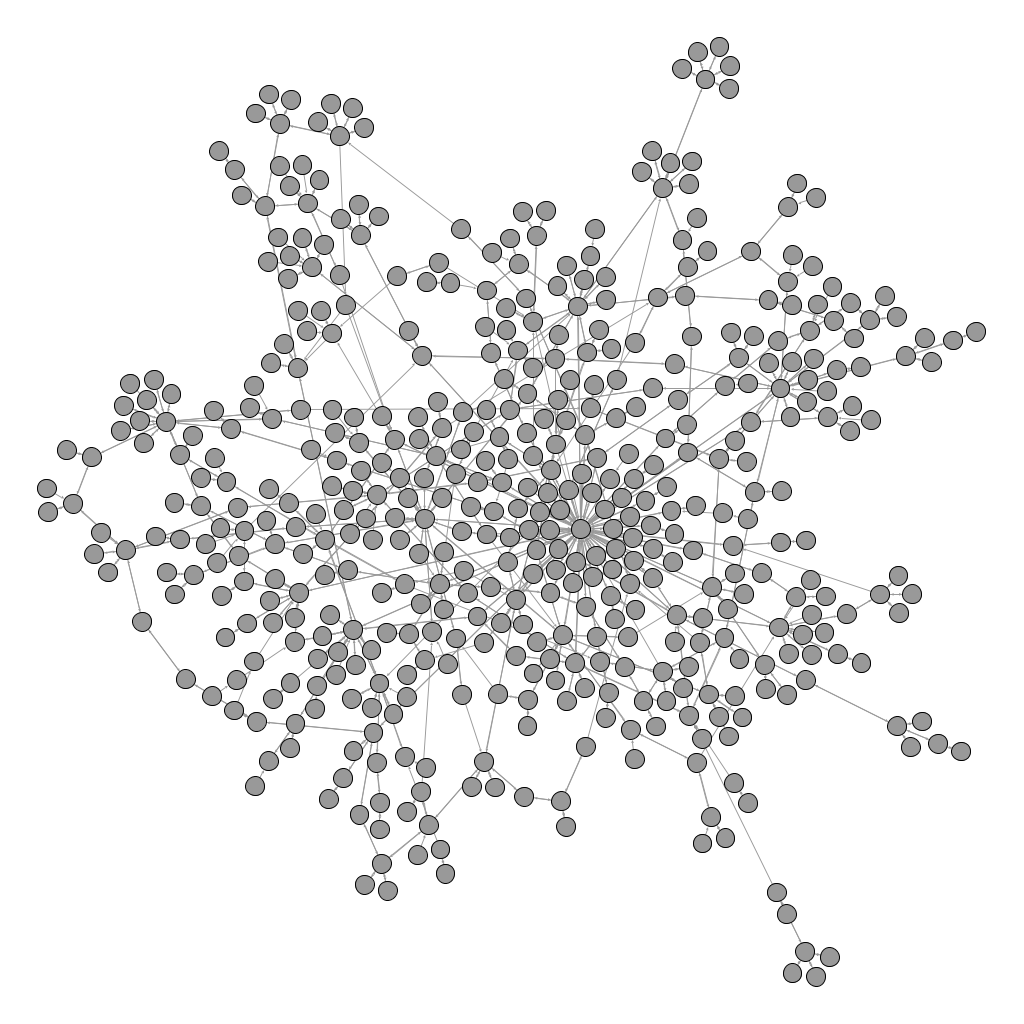
\includegraphics[scale=0.25]{example-graph.png}
\end{center}
\caption{Example Network Representation}
\label{img:ex-graph}
\end{figure}

It was decided that the graph should be directed in order to to better model a relationship as undirected edges only indicate a connection, whereas directed edges reveal much more. This works on the principle that a friendship is not necessarily mutual since one person may consider another a friend whilst the other may not reciprocate. Due to this, an edge from node A to node B represents `has a relationship with' and by extension `influences' as seen in figure \ref{img:ex-edge}.

\begin{figure}
\begin{center}
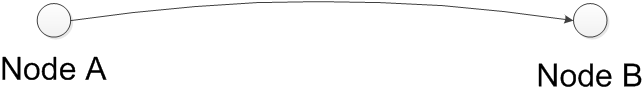
\includegraphics[scale=0.5]{example-edge.png}
\end{center}
\caption{Example Edge: Node A influences Node B}
\label{img:ex-edge}
\end{figure}

\subsubsection{Influence}
The concept of \emph{influence} is modelled in a manner similar to a probability; it is a weight on an edge with a value between 0 and 1, where 0 represents no influence and 1 represents absolute influence. In general, this makes it easier to calculate multi-hop influence and influenced attributes; in doing so it drastically reduces the complexity of operations carried out on a regular basis over multi-value or object-based approaches. Rather than emulate relationships and their influences at a more complex level, this basic approach was judged more reasonable since it would not require further conversion when it interacts with other elements of the model. 

Importantly, this implementation of influence remaps the concept of positive and negative opinions of a person to a linear scale, for example a person may dislike another, causing them to not want to take on their traits. As such, a negative figure should be relating to a low influence value and a positive one being seen as holding a higher influence.
\emph{Multi-hop influence} within the model aims to recreate the idea of `friends-of-friends', with the belief being that should the friends of an individual are influenced by a third-party, that party should, in turn, influence the individual in some way. In the graph, this is represented by a series of edges from one node to another, as seen in figure \ref{img:multihop-inf}. The extent to which this influence acts on the individual is a matter for tuning of the model and will be discussed in the agent description (Section \ref{sec:agent}). Obviously, the influence at one hop is simply the weight of the influencing edge, whereas to calculate the influence at $n$ hops, the formula \ref{eq:multihop-inf} is used, where $w_{i}$ is the influence value of an edge, $w_{0}$ is the edge to the current node and the route from $0$ to $n$ (seen in figure \ref{img:multihop-inf-calc}. By multiplying the influence of each hop together, a likeness to weakening influence across the mutual friends is incorporated along with the method giving a probability-alike value that can be used when calculating influenced attributes. A common situation may be that there are a number of routes to a given destination node from a source and as a result, a number of possible influence values for this `friend-of-a-friend'. Once again, simplicity is maintained by taking the highest value - this is based on the assumption that the higher value represents a chain of stronger influences (i.e. friendships) and due to this, a person is likely to opt for that input rather than the ones of weaker influence.

\begin{figure}
\begin{center}

\includegraphics[scale=0.75]{multi-inf.png}
\end{center}
\caption{Indirect Influence: Influence Across Multiple Hops}
\label{img:multihop-inf}
\end{figure}

\begin{equation}
\prod_{i=0}^{n}w_{i}
\label{eq:multihop-inf}
\end{equation}

\begin{figure}
\begin{center}
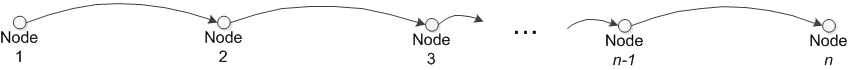
\includegraphics[scale=0.75]{multihop-inf.png}
\end{center}
\caption{Calculating Influence Across Multiple Hops}
\label{img:multihop-inf-calc}
\end{figure}
\emph{Influenced attributes}, in this model, are defined as how an individual perceives the actions of another affecting themselves with the intention being that the influence provides some form of weighting against the actual value of the attribute. As will be described in section \ref{sec:neighbourhood}, part of the agent definition, the idea is for an agent to have an `ideal agent' to which they move towards, where the attributes for this figure are calculated using averages of these influenced attributes. In regards to calculating the attributes, the general formula used can be seen in equation \ref{eq:inf-attr} where $N$ is the neighbourhood (defined in Section \ref{sec:neigh}) of the current node, $\text{\emph{attribute}}_{n}$ is an attribute value and $\text{influence}_{n}$ is the influence of that node. There were a number of changes that were required for some data types but, since these depend on the specific attribute they will be detailed in section \ref{sec:agent}.

\begin{equation}
\frac{\sum_{\forall n \in N} \text{\emph{attribute}}_{n} \times \text{\emph{influence}}_{n}}{\sum_{\forall n \in N}\text{\emph{influence}}_{n}}
\label{eq:inf-attr}
\end{equation}
From both multi-hop influence and influenced attributes, it can be seen that there is not a direct representation of negative opinion causing a person to act in an opposite manner to the figure they dislike. This is a move away from a realistic behaviour as generally, it would be expected for someone to avoid behaving like a person that they do not get along with though including this would require some form of state in the relationships between nodes to be maintained. Since it was decided that weighted edges were a simple but expressive method and that storing state on these is difficult, requiring a great deal of extra computational complexity on each turn, it was omitted.

\subsubsection{Graph Generation \& Sampling}
\label{sec:GGS}
As described in the platform description (Section \ref{sec:platform}), a number of graph generation and sampling methods are available to provide networks for use within a simulation. Since this system is designed to simulate upon smaller networks than a commercial environment might, using large, real-world networks is not always ideal. This is because networks of many thousands of nodes, each requiring many operations to work out influence, attributes and decisions, causes simulations to last for a very long time. An alternative was required that could provide a number of realistic but smaller networks for the simulations.

\emph{Scale-free} networks were included due to their regularity of appearance within social circles – typically, they provide a low-to-medium edge density across nodes, with a number of hub nodes~\cite{BA-SciAm}. This is particularly useful since it allows the investigation of `social hubs' within a network to see whether this kind of figure has a specific effect on the smoking behaviours of those around them. A disadvantage with this type of network is that, on the examples generated for this project the average node tended to have a fairly low degree. Since edges represent relationships, it could be argued that it is not representative of a realistic group. To counter this, nodes within this graph could be considered as groups of humans (and in effect a small-world network) or simply a less dense friendship group, such as an office of workers, where ties are more likely to show acquaintance than friendship. As an aside, this type of graph was most useful for testing the model on since it clearly exhibited any signs of imbalance or lack of change over a number of simulation steps. An example scale-free graph can be seen in figure \ref{img:ex-scale-free} with the generation algorithm being given in figure \ref{code:sf-code}.

\begin{figure}
\begin{center}
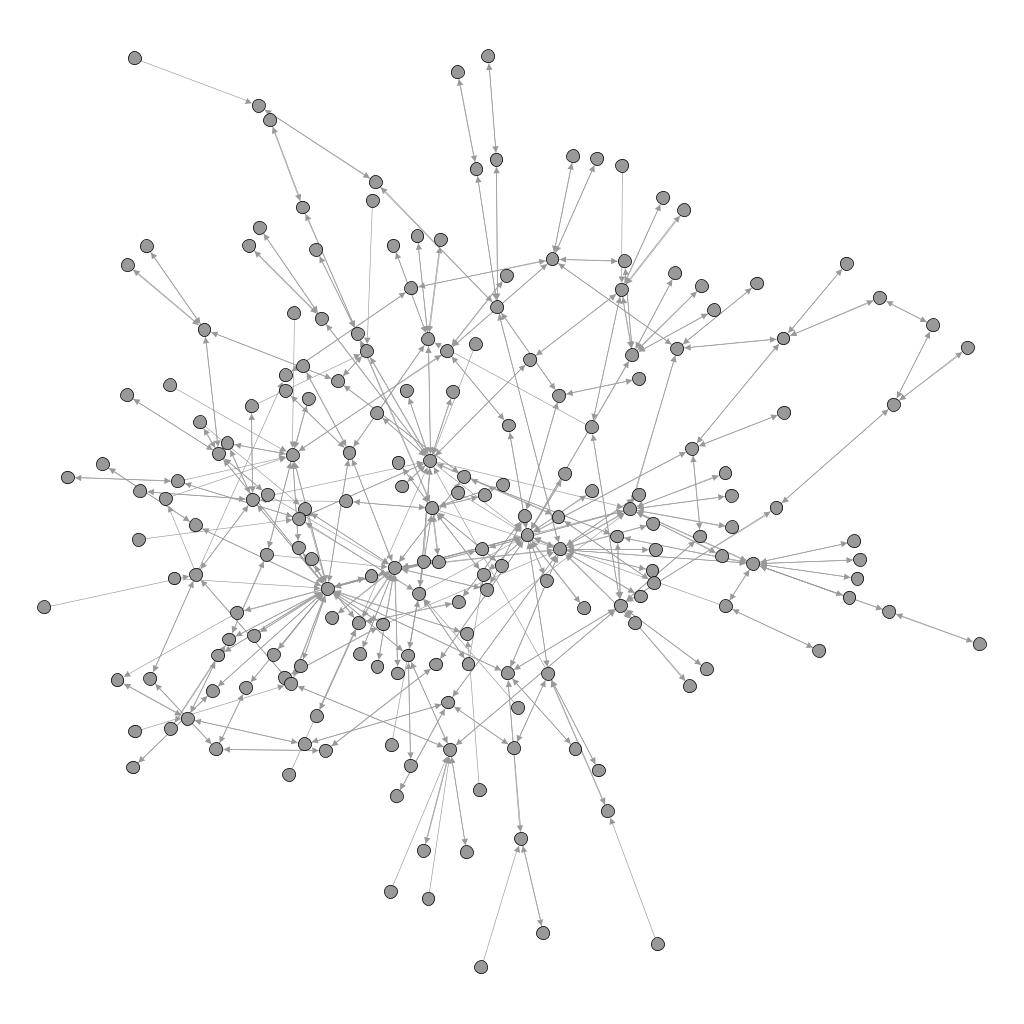
\includegraphics[scale=0.4]{ex-scale-free.png}
\end{center}
\caption{Example Scale-Free Graph with 196 Nodes}
\label{img:ex-scale-free}
\end{figure}

\begin{figure}
\begin{enumerate}
\item Begin with a graph of $m_{0}$ nodes, where $m_{0} \geq 2$ and each node has degree of at least 1.
\item Add new nodes incrementally. For each new node consider connecting to each other node $i$ with the probability $p$, calculated using equation \ref{eq:SF-formula} where $k_{i}$ is the degree of $i$.
\end{enumerate}
\caption{Generation Algorithm for Scale-Free Graphs by the Barab\'{a}si-Albert Model~\cite{BAStat}}
\label{code:sf-code}
\end{figure}

\emph{Small-world} networks are another useful inclusion; the main aim with this type of network was to be able to simulate the effects of groups of close friends like one might find in a club or society~\cite{small-world}. In general, a small-world network displays high connectivity relative to the number of nodes present (assuming that the mean number of edges it is generated with is of reasonable size). The key downside of this method is that due to the raised level of connectivity, the chance of small feedback loops forming is much higher than scale-free networks. This can cause imbalance within the simulation due to nodes influencing each other to take on more extreme behaviours and thus exuding this influence to their respective neighbours. As a result, this type of network should be used with caution and balanced carefully to avoid these situations. When small-world networks are used, the relevant balancing will be stated. Figure \ref{img:ex-small-world} shows an example small-world network with figure \ref{code:sw-code} displaying the generation algorithm.

\begin{figure}
\begin{center}
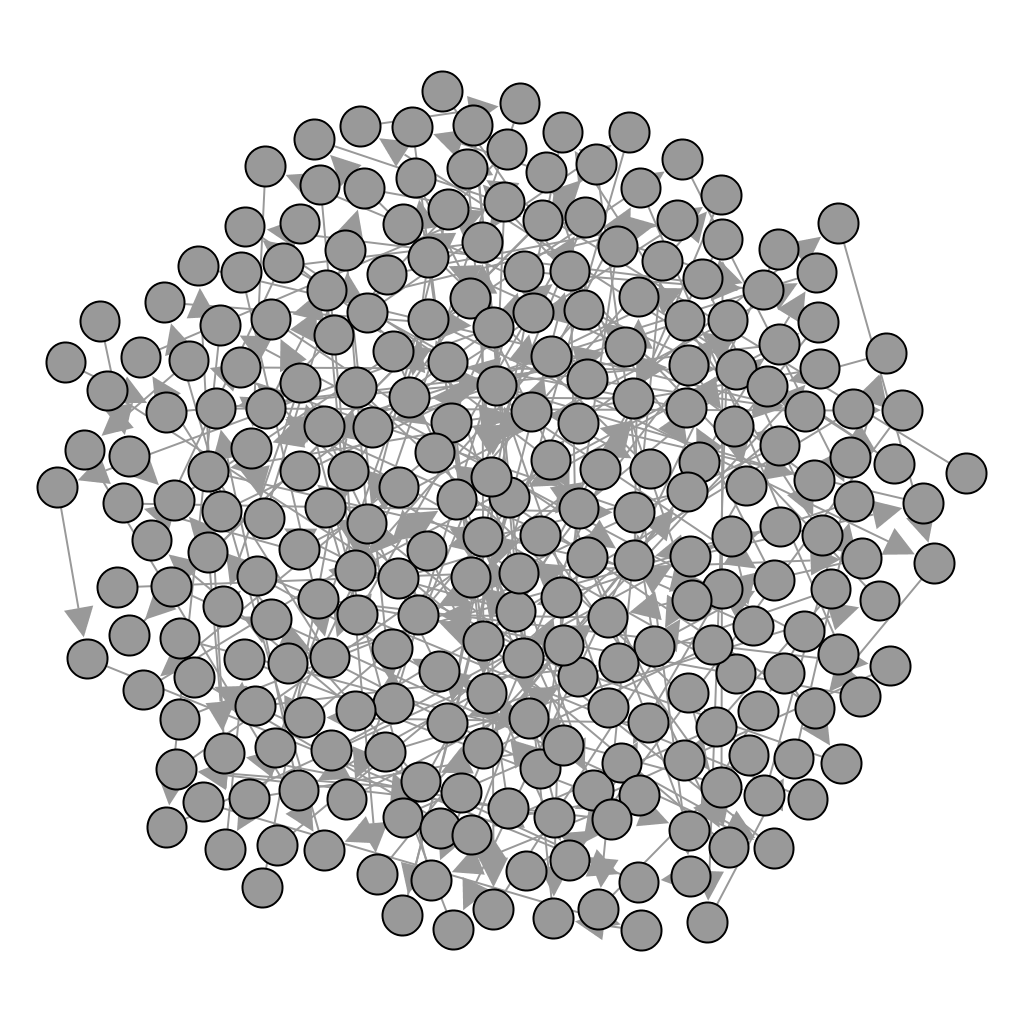
\includegraphics[scale=0.25]{ex-small-world.png}
\end{center}
\caption{Example Small-World Graph with 250 Nodes}
\label{img:ex-small-world}
\end{figure}

\begin{figure}
For building a network of $N$ nodes, mean degree $K$ and a value $\beta$, where $0 \leq \beta \leq 1$ :
\begin{enumerate}
\item Create a ring lattice of $N$ nodes where each node is connected to its first $K$ neighbours, where it has $\frac{K}{2}$ on each side. For a sparse but connected network, $N \gg K \gg \ln{N} \gg 1$.
\item For each node in the graph, consider each of its edges that connect to yet-unencountered nodes and rewire that edge to connect to a randomly chosen node with probability $\beta$, not allowing self-connection or duplicate edges.
\end{enumerate}
\caption{Generation Algorithm for Small-World Graphs by the Watts-Strogatz Model~\cite{BAStat}}
\label{code:sw-code}
\end{figure}

\emph{Snowball sampling} was the chosen method for real-world graph sampling, due to its simplicity in terms of implementation. Because of the nature of this sampling method, one of a breadth-first search from a random node, it characteristically produces graphs that have one major hub from which most edges emerge. Due to the fact that it can be run on graphs sampled from real-world social networks, the product is often a mix between what might be expected of small-world and scale-free networks. Whilst this was not particularly useful for developing the model upon due to the often high level of connectedness, it does allow for a much wider range of tests to be carried out using the system. This tool is included primarily for the sampling of real-world networks since sampling generated networks is simply replaced with generating networks of the required size. Instead, the number of nodes required can be extracted from datasets sampled from social networks, giving the simulation the ability to run on real graphs. An example of a snowball sample can be seen in figure \ref{img:ex-snowball}, gathered from an email dataset by the \emph{SNAP} project~\cite{SNAP-email}

\begin{figure}
\begin{center}
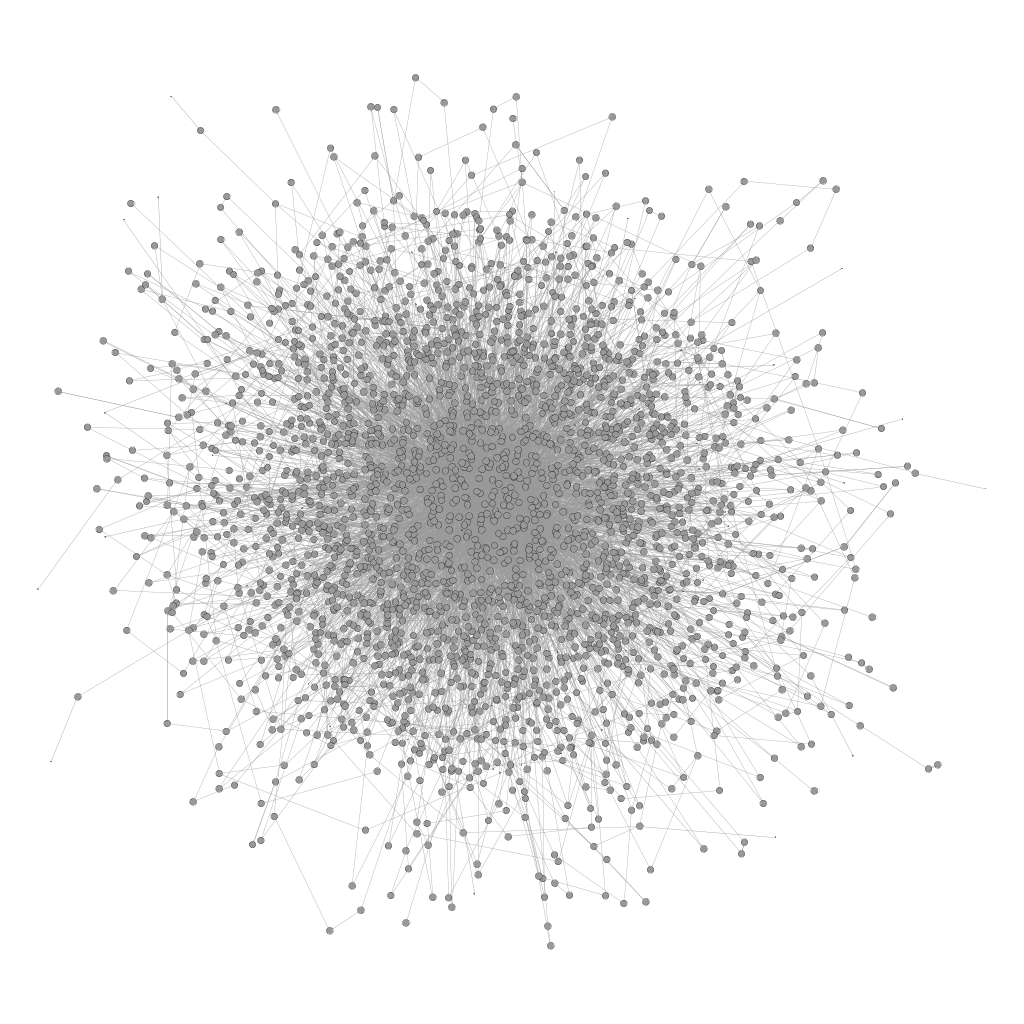
\includegraphics[scale=0.4]{ex-snowball.png}
\end{center}
\caption{Example Snowball Sample Graph with 2790 Nodes}
\label{img:ex-snowball}
\end{figure}

\subsubsection{Graph Stability}
In the early stages of development a regular occurrence was for the graph to, exhibit very high clustering coefficients for a number of nodes, due to actions undertaken by agents. This was caused by many agents interacting on a regular basis, the complexity of which it was too difficult to balance entirely through careful parameter selection and agent action changes. In order to maintain this a balance, the \emph{WatchMan} was used to intervene should the graph become too clustered.

The way in which intervention was judged necessary had an effect on the workings of the network and to account for this, two different methods were implemented and tested. The first of these takes the average clustering coefficient of all nodes in the graph and, if above a threshold set as a system parameter, 10\% of the nodes in the graph ordered by highest clustering coefficient first have each edge (both in- and out-) considered for removal with a 50\% chance. Whilst an artificial way to maintain balance, it did provide a more stable graph since thinning out edges on the nodes central to the clusters reduces the number of feedback loops, which helps to slow the compression of the network.

The other method was to choose 10\% of the nodes from the graph at random and calculate the average clustering coefficient at one hop for each. If over a separate simulation parameter threshold to the above, they are stored as a locally high clustering coefficient node. Each of these nodes is then analysed in a similar manner to the previous method, in that they have each of their edges considered for removal with the chance of this happening at 50\%. This is a more targeted approach that aims to prevent strongly-bound clusters forming at an earlier stage by again thinning out their ties. In testing, the value of the threshold was revealed to be very important as due to the `early stage' prevention of heavy clustering, the removal could become overzealous and make the graph sparse. By increasing the threshold for a node to be classed as a locally high clustering coefficient, this method is reserved for only extreme cases.

To illustrate the effects of these stability measures, figure \ref{img:pre-watchman} displays how a non-stabilised graph may appear after 120 steps compared to the stabilised version, figure \ref{img:post-watchman} at around 120 steps. Even though the external intervention does mean that the model loses some faithfulness to real-world interaction in respect to balance, the fact that the network can provide much more useful results by running longer simulations outweighs this. Furthermore, to have the model balance itself through the interactions themselves would require a significantly more involved representation of agent networking with a lot of time spent on balancing, which is beyond the scope of this project.

\begin{figure}
\begin{center}
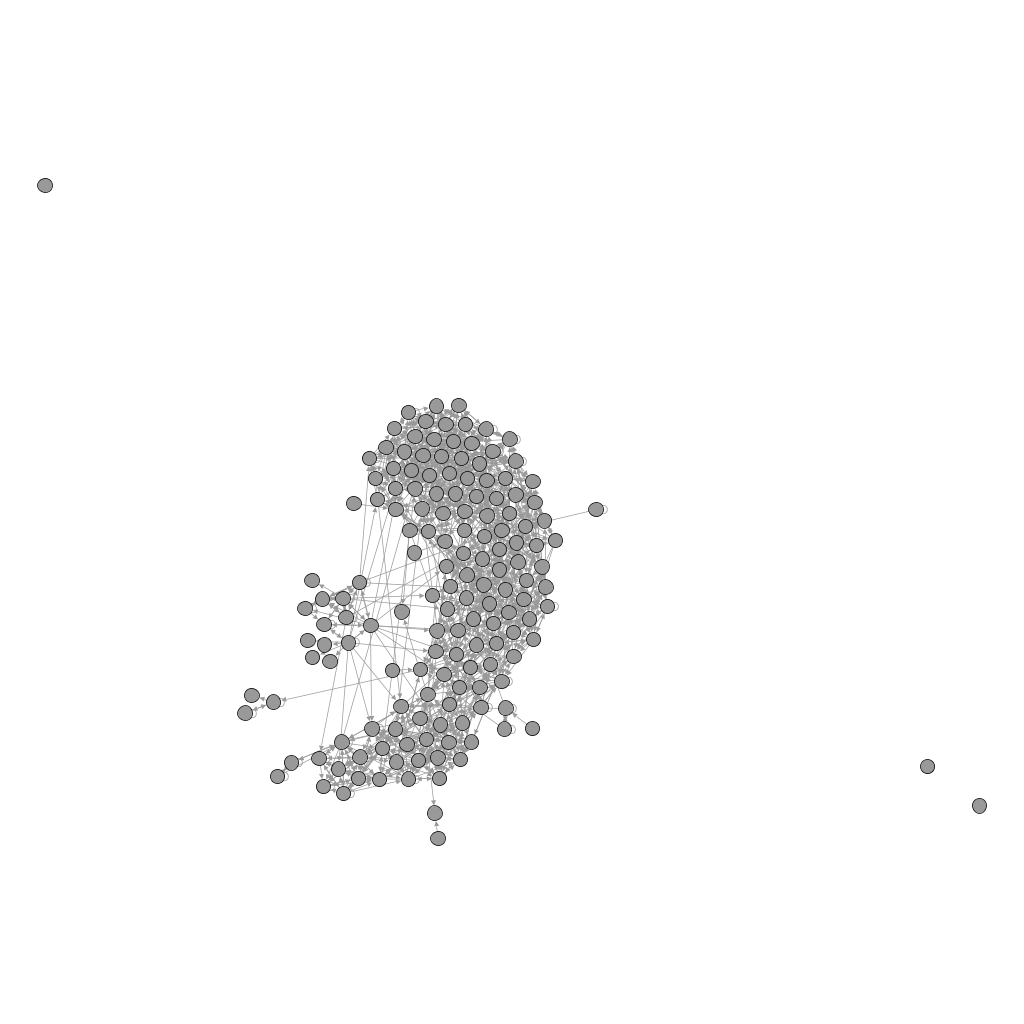
\includegraphics[scale=0.4]{pre-balance.png}
\end{center}
\caption{Unstable Graph with 155 Nodes}
\label{img:pre-watchman}
\end{figure}

\begin{figure}
\begin{center}
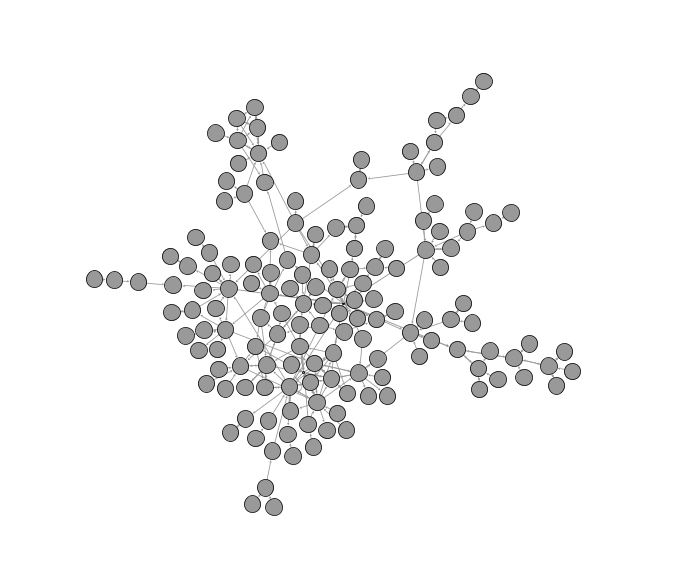
\includegraphics[scale=0.5]{post-balance.png}
\end{center}
\caption{Stable Graph with 152 Nodes}
\label{img:post-watchman}
\end{figure}

\subsection{Agent}
\label{sec:agent}
The agent was the most significant section of the project in both function and time taken to build. Within this section of the model, decisions are made about how to change behaviours, influence is acted upon and connections to other nodes are reconfigured; since the social network provides the framework within which the agents act, most of the ability to tune the model arises through various aspects of the agent. It is split into two sections: \emph{attributes}, the data that defines the agent and by extension, the human, and \emph{actions} which are the functions that an agent can perform in a simulation step.

The basic principle for the agent is that within their \emph{local neighbourhood}, i.e. the nodes that they are within one hop of, influence is used to generate an `ideal person'. This figure is a set of attributes that is effectively the `average' of this neighbourhood and to which the agent in question would apsire. Using both these attributes and a number of metrics about the surroundings, the agent then follows a decision tree which provides the chance for an attribute change. On the back of this, the agent can reconfigure their social connections based on their current attributes, scoring themselves against others in their neighbourhood.

Throughout the development of the model, testing was carried out by running the simulation on a scale-free graph and observing how it behaved. In general, the expected behaviour was for the network to avoid collapsing into a feedback loop and/or having a high average clustering coefficient whilst displaying some change. This was considered to be an indication of a balanced model, which is an aim of the project – an example of both a balanced and imbalanced model can be seen in figures \ref{img:ex-simbase}, \ref{img:ex-noncrunch} and \ref{img:ex-crunch}, the difference between the latter two being that the imbalanced network has an extremely high concentration of edges in one sub-area whereas the balanced network has a more distributed concentration.

\begin{figure}

\begin{center}
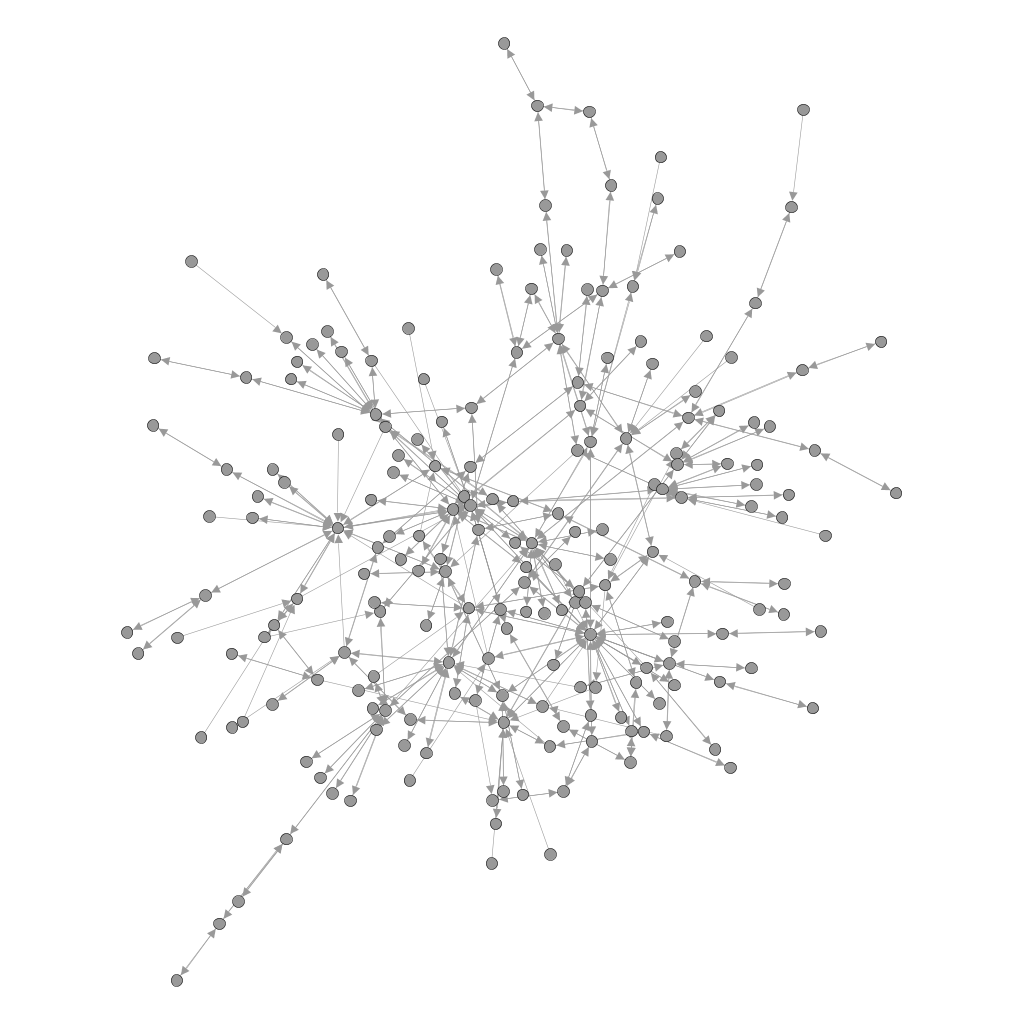
\includegraphics[scale=0.4]{simbase.png}
\end{center}
\caption{Baseline Graph with 196 Nodes}
\label{img:ex-simbase}
\end{figure}

\begin{figure}
\begin{center}
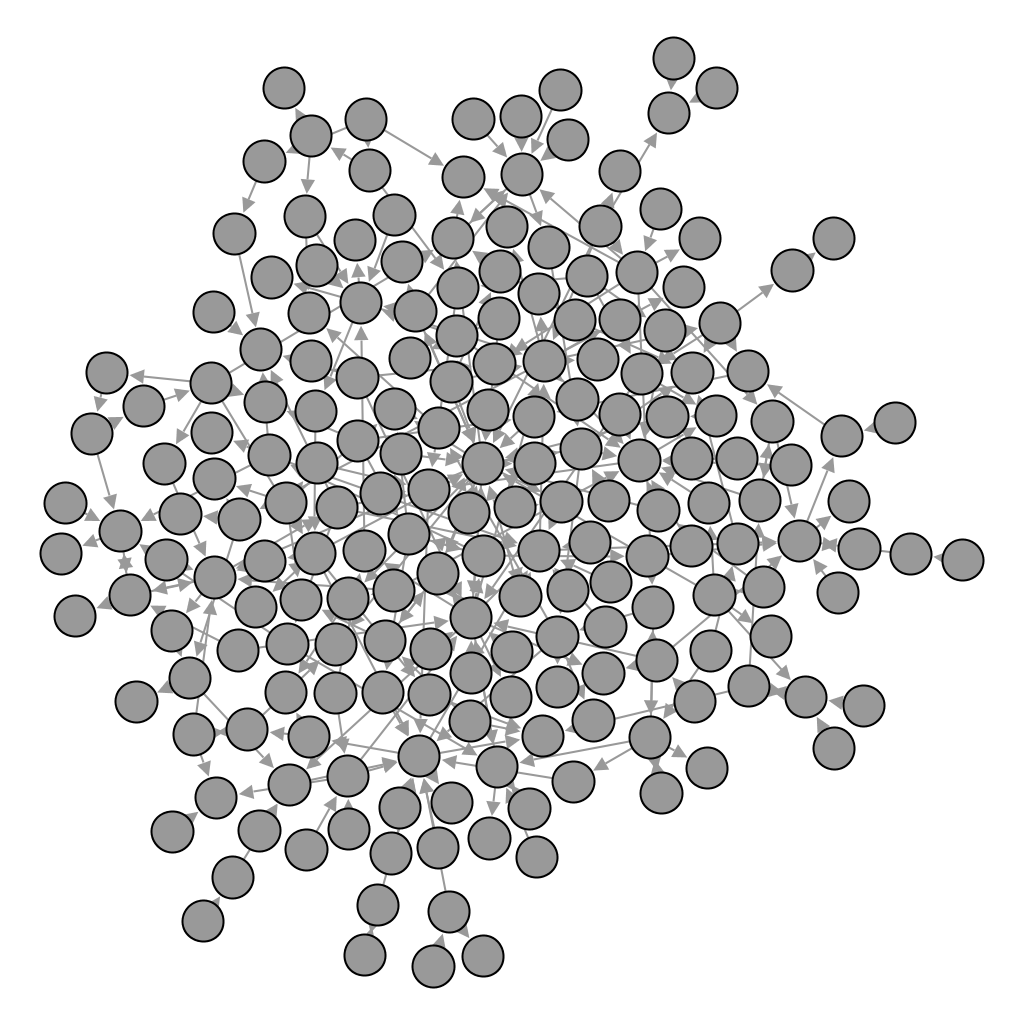
\includegraphics[scale=0.25]{non-crunch.png}
\end{center}
\caption{Balanced Graph with 196 Nodes}
\label{img:ex-noncrunch}
\end{figure}

\begin{figure}
\begin{center}
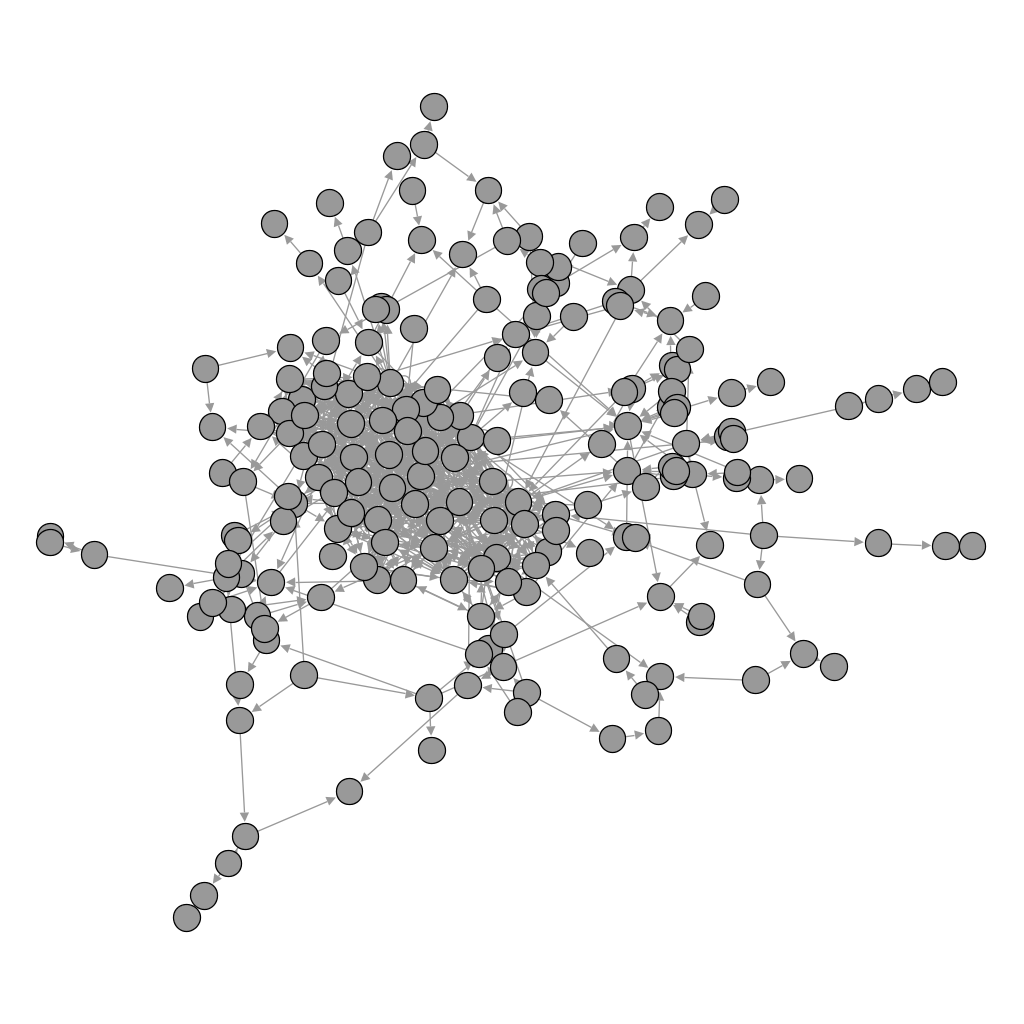
\includegraphics[scale=0.25]{crunched.png}
\end{center}
\caption{Imbalanced Graph with 196 Nodes}
\label{img:ex-crunch}
\end{figure}


\subsubsection{Attributes}
Many attributes were considered with the intention of modelling human smoking behaviour as accurately as possible, however this is a difficult notion due to the lack of detailed information relating about smoking cessation. A large part of the information that does exist, such as NHS statistics~\cite{NHS-43}, is based on survey information which in turn may bring an element of bias. Generally speaking, the attributes were added on an ad-hoc basis in the early stages of development; once an idea of the type of factors involved in smoking cessation were known through research, specific ones were implemented on the basis of simplicity and usefulness within the model.

Initially, a number of attributes were considered that extended the smoking cessation decisions into areas of lifestyle such as alcohol consumption and stress~\cite{NHS-44}~\cite{malay}. Early on in development, it was decided to avoid using these since the methods to simplify and represent them would remove a large part of the usefulness – for example representing stress would require two functions, one to map produce values for stress caused externally to the system and one for stress as a result of the actions chosen. This is a complicated endeavour since modelling stress in itself is field worthy of research. A similar decision was made for alcohol consumption as attempting to model factors such as social smoking when under the influence of alcohol is difficult and again could be the focus of a modelling project itself.
The attributes chosen for the agent can be seen in table \ref{tab:attr}.

\begin{figure}
\begin{center}
\begin{tabular}{|l||l|p{5cm}|p{5cm}|}
\hline
\bf{Name} & \bf{Type} & \bf{Lower of Range Represents} & \bf{Upper of Range Represents} \\
\hline
\emph{isSmoker} 					& Boolean & \emph{False} - Does not smoke											& \emph{True} - Smokes \\
\emph{willpower}					&	Double	&	\emph{0} - Has no resistance to change							& \emph{1} - Has high resistance to change \\
\emph{health}						&	Double	&	\emph{0} - Is of very poor health e.g. has disease &	\emph{1} - Is of perfect health \\
\emph{smokedPerDay}			&	Integer	&	\emph{0} - No cigarettes per day										& \emph{70} - 70 cigarettes per day \\
\emph{givingUp}					&	Boolean	&	\emph{False} - Is not giving up smoking						& \emph{True} - Is giving up smoking \\
\emph{giveUpAttempts}		&	Integer	&	\emph{0} - No previous attempts at giving up				& No upper limit \\
\emph{stepsSinceGiveUp}	&	Integer	&	\emph{0} - No simulation steps since giving up began/is not giving up	& \emph{500} - Simulation steps since giving up began \\
\emph{sociable}					&	Double	&	\emph{0} - Is a social recluse											& \emph{1}	- Is an extrovert \\
\emph{influenceability}	&	Double	&	\emph{0} - Is not easily influenced								& \emph{1} - Is easily influenced \\
\hline

\end{tabular}
\end{center}
\caption{Description of Agent Attribute Types and Ranges}
\label{tab:attr}
\end{figure}


The most basic attribute is that of \emph{isSmoker}, which simply shows if an agent is currently a smoker or not. This is coupled with \emph{smokedPerDay}, representing the number of cigarettes smoked per day, form the fundamental smoking behaviour in the model. The number of cigarettes smoked per day is very important since statistics indicate that heavy smokers, those smoking over 20 cigarettes a day, are less likely to want to quit than lighter smokers~\cite{NHS-43} which is crucial in deciding whether an agent should give up. As can be seen in the table, there is an upper cap on this value; since feedback loops are almost inevitable in the system  - and may be natural in real-world networks - this cap prevents one feedback loop causing excessive damage to the rest of the environment. In early tests without the cap, it was not uncommon for agents to be smoking upwards of 1000 cigarettes per day due to a few nodes influencing others with their higher than average smoking rates, in turn spreading this throughout the network. Although the cap is artificial, it in some way maps to a physical limit of cigarettes smokeable in a day.

\emph{Health} is another important inclusion as the quality of a person's health impacts their views of smoking and their likeliness to continue~\cite{NHS-43}. Although only a basic method of including health in the model, using a value between 0 and 1 means that it can act in a similar manner as a probability. In a commercial model, this attribute could be implemented in a much more detailed way, including types of illness, how developed an illness is and a more accurate function of how health quality changes over time. There is a strong interplay between the status of the agent as a smoker and the change in health. Since the health in this model is in respect to smoking-related illness, being a smoker decreases health slightly on each turn, whereas being a non-smoker increases it.

Three separate attributes handle the process of giving up. As indicated in the research for this project, those who are in the process of giving up smoking are likely to relapse and restart smoking~\cite{NHS-44}; being able to incorporate for how long someone has been giving up models the process more accurately. The \emph{isGivingUp} field stores whether an agent is in the process of giving up and can only be true when that individual is not a smoker. Furthermore, to simulate the giving up period, \emph{stepsSinceGiveUp} is set to 0 whenever a giving up attempt is started and incremented on every simulation step. Obviously, a point arises where the individual no longer considers themselves to no longer be someone `giving up' and instead just a non-smoker. The simulation does this by limiting the number of steps someone `gives up' for, and at that point sets \emph{isGivingUp} to false so that the effect of attempting to quit no longer impacts on the choice to relapse into smoking. A final aspect is that of the number of attempts at giving up someone has. Again indicated by the NHS statistics, those who have attempted to give up smoking and failed before are more likely to fail again~\cite{NHS-44}. By tallying the number of giving up attempts to date (incremented every time an agent changes \emph{isSmoker} from \emph{false} to \emph{true}) this can be factored in to the decision tree.

The final attributes are those of \emph{sociability} and \emph{influenceability}. Again values between 0 and 1, the former attempts to represent some aspect of willingness to form new social connections. Although not directly related to smoking cessation, it adds an individual trait to agents for reconfiguring their connections. The latter, how easy the person is influenced, is used as an extra factor in deciding when agents change their behaviour, i.e. give up/begin smoking, to model the idea that in order for those who reject most influence would require a lot of sustained pressure to take on the influenced behaviour. In addition to this, it provides two extra attributes for comparison of agents, specifically in terms of assessing similarity, as people who seek social connections will naturally be more likely to connect to others who are doing the same.

In terms of assigning values to these attributes, a normal distribution was widely used for numerical attributes. Due to the abstraction of the attributes - representing largely unquantifiable concepts with decimal numbers - determining appropriate values for the means and standard deviation was a matter of balance for the model. By including the mean and standard deviation sets for all attributes as system parameters, they can be adjusted through different simulations allowing for analysis into how this affects the network.  Generally, opting for a mean of around 0.5 and a standard deviation of 1 provides a reasonable spread of values across the agents. For the Boolean attributes of \emph{isSmoker} and \emph{isGivingUp}, system parameters specify the probability for each being true with uniform random numbers being tested against them. Again, this allows for the user to investigate different starting states of the simulation with regard to the number of smokers/non-smokers present.

\subsubsection{Action Overview}
In regards to the `rules' section of this agent, there are three parts to each simulation step. First, the agent calculates a series of metrics in regards to its surrounding nodes, then uses these as part of a decision process organised into a decision tree. A decision tree can be described as a tree structure where the nodes are decisions to be made and branches are different options for a given decision. This allows the agent a chance to modify its own attributes and from there reconfigure its connections to other nodes, if necessary.
\subsubsection{Neighbourhood Actions}
\label{sec:neigh}
In the network, every agent connected to one or more other node has a \emph{neighbourhood}. This is defined to be the set of nodes that can be reached within $n$ hops, where $n$ is a parameter to the simulation. This represents the concept of influence through `friends-of-friends' and the assumption was made that $n=2$ was a more resonable choice since during development,  graphs of hundreds, rather than thousands, of nodes tended to have an average path length of less than 10. Requiring nodes to draw upon more than a two-hop neighbourhood would result in a much larger portion, in terms of node count and network diameter, of the whole network impacting a node. To avoid a case of very distant nodes playing too much of a role in influence, $n$ was kept low. In terms of attributes calculated using this neighbourhood, figure \ref{tab:neighbour} provides more information.

\begin{figure}
\begin{center}

\begin{tabular}{|l||l|p{10cm}|}
\hline
\bf{Name} & \bf{Type} & \bf{Represents}\\
\hline
\emph{infIsSmokerVal} 	& Double 	&	The calculated influenced attribute of \emph{isSmoker}, with $\leq 0$ being false and $\geq 0$ being true.									\\
\emph{infIsSmoker}			&	Boolean	&	A boolean value representing the outcome of \emph{infIsSmokerVal}							\\
\emph{infHealth}				&	Double	&	The influenced attribute of \emph{health} \\
\emph{infWillpower}		&	Double	&	The influenced attribute of \emph{willpower}										\\
\emph{infCigPerDay}		&	Double	&	The influenced attribute of \emph{smokedPerDay}						\\
\emph{avgCigPerDay}		&	Double	&	The average of all non-zero \emph{smokedPerDay} values in the neighbourhood				\\
\emph{pcSmokes}				&	Double	&	The percentage of neighbours who smoke\\
\emph{pcGivingUp}			&	Double	&	The percentage of neighbours who are giving up smoking (and are not just non-smokers)\\
\emph{infPcSmokes}			&	Double	&	The influenced percentage of neighbours who smoke								\\
\emph{infPcGivingUp}		&	Double	&	The influenced percentage of neighbours who are giving up							\\
\hline
\end{tabular}
\end{center}
\caption{Description of Agent Attribute Types and Ranges}
\label{tab:neighbour}
\end{figure}

Aside from the `ideal agent' attributes that are calculated for the current agent, a number of figures that describe the current basic state of those in the neighbourhood are calculated. Percentages of the graph which smoke and are giving up are particularly useful in creating the effect of peer-pressure within decisions, as well as being a possible representation of what the agent would be surrounded by in their life. This can be furthered by including the influence of the surrounding nodes into these percentages, which can be seen in formula \ref{eq:inf-perct} where $n$ is a neighbourhood node, $s$ a node of a specific dispositon (e.g. a smoker) and $n_{i}$ being the influence of $n$. This enables the system to attempt to model situations where a person's susceptibility to peer pressure depends on how influential those surrounding them are; should they be of low influence, it is unlikely that the person would adopt a behaviour that they are displaying.

\begin{equation}
\label{eq:inf-perct}
\frac{\sum_{\forall s \in N} s_{i}}{\sum_{\forall n \in N} n_{i}}
\end{equation}

As described previously, the compound influence across a multi-hop route can be calculated so from this, the influence to each node within the neighbourhood can be gathered. Using this information, the `ideal figure' for this neighbourhood is then produced using influenced attributes by effectively averaging attributes over all of the nodes in the neighbourhood. The way in which influence attributes are calculated is slightly different for Boolean variables but in general, formula \ref{eq:inf-perct} is used. Booleans instead have values of true mapped to 1 and false to -1 to allow for influence to be worked into the `ideal person'. Once summed over the whole neighbourhood, a negative value indicates \emph{false} and positive \emph{true}. Notice that the sum of $\text{\emph{influence}} \times \text{\emph{attribute}}$ is divided by the total influence, not the number of nodes. This is because, through experimentation, division by the number of nodes resulted in very low values for influenced attributes whereas using the sum of influence gave typically more reasonable figures. Due to this, it is less a normal average, instead weighted based on the influence of a node. It should be noted that this will never exceed the values that would be generated by simply averaging out attributes since that would be a case where all nodes were at an influence of 1. Another point to note is that when calculating with influenced \emph{smokedPerDay}, cases of non-smokers (i.e. those who smoke no cigarettes) were excluded to avoid artificially lowering the average.

\label{sec:neighbourhood}

\subsubsection{Decision Tree Actions}
\label{sec:dectree}
In order to change their own attribute values, an agent must go through a series of decisions to choose which value to change. The aim of this approach is to model a human decision making process in a logical and maintainable way, so that decisions can be rearranged, inserted or removed easily. In general, more important decisions are placed higher in the tree since they are more likely to be reached by an agent than any decision lower in the tree, by which point the decision in question becomes one in many. Because of this, when the importance of decisions is discussed those of higher importance will be referred to as higher in the tree than ones of lower importance. Throughout the development, a major focus was to uphold balance within the tree. This means that where possible, feedback loops causing extreme attribute values should be minimised and excessive clustering within the network should be avoided. Both of these had to be monitored by testing different versions of the decision tree, with changes being made as necessary.

To begin with, an approach was taken to combine a number of attributes into calculations that can be seen in figure \ref{eq:v0.9probs}, the labels referring to points in the tree as seen in figure \ref{img:init-dectree}. Generally, the tree was kept fairly shallow in favour of producing values for manipulating attributes, similar to probabilities or range checks. For example, in figure \ref{eq:v0.9probs}, \emph{B} shows how the decision is made based on whether the agent attributes are within 10\% of the influenced attributes – if so, the number of cigarettes smoked is adjusted. As each decision required such a combination, to build a sufficient series of decisions the same parameters would have to be formed in different ways for each choice. It became clear that this approach was flawed as it lent itself into collapsing many separate attribute choices into one. This lost control over how each parameter effects the end choice and made it very difficult to add new decisions as most were already represented in some way in the existing steps. Furthermore, using combinations of attributes led to extra complexity making it unclear exactly which attributes are causing different effects. Since a substantial part of this project is to understand what the model is showing, difficulty in isolating attributes and judging their effects is problematic. As a result, the decision tree was heavily separated out into single attribute decisions that lead into one another.

\begin{figure}

	$\forall n \in N$ where $N$ is the Neighbourhood of a node:
	\begin{enumerate}
		\item p(\emph{give up smoking})=$(1-health_{n}) \times \frac{|\text{Nodes giving up smoking}|}{|\text{Nodes}|}$ \\
		\item If $n$ smokes $\pm10\%$ of the influence sum for \emph{cigarettes smoked per day}, and $\text{\emph{health}}_{n}$ is within $\pm10\%$ of the influence sum of \emph{health}. \\
		\item $change = (\text{influence sum of \emph{smoked per day}} - {smokedPerDay}_{n}) \times influenceability_{n}$, else there is no change. \\
		\item p(\emph{take up smoking}) = $health_{n} \times \frac{|\text{Nodes giving up smoking}|}{|\text{Nodes}|} \times \frac{|\text{Nodes who smoke}|}{|\text{Nodes}|}$ \\
		\item If the influenced sum of the \emph{number of cigarettes per day} is $< 0$, then $smokedPerDay = 5$, otherwise \\
		$smokedPerDay = \operatorname{round}(\frac{\sum_{\forall n \in Neighbours} smokedPerDay_{n} \times influence_{n}}{\sum_{\forall n \in N} influence_{n}})$
	\end{enumerate}
	\caption{Initial Decision Tree Probability Calculations}
	\label{eq:v0.9probs}
\end{figure}

An example of the results of the transformation that took place can be seen from \emph{equation 4} in \ref{eq:v0.9probs} to figure \ref{img:example-decision}, where each part of the combined decision is put into a `level' of the new tree with some stages being removed. By doing this, not only is the tree more structured and manageable but decisions can be traced through each branch revealing how different configurations can affect the decision making. The overall result of this stage was to move the tree from figure \ref{img:init-dectree} to figure \ref{img:0.9-dectree}. The values on each edge in figure \ref{img:0.9-dectree} represent the thresholds that need to be matched for that branch to be followed.

It is worth noting the inclusion of an \emph{irrational choice}, as seen in figure \ref{img:example-decision}. This is to add a human characteristic into the simulation and introduce a small element of unpredictability. The probability of an irrational choice is a simulation parameter so can be changed easily. Importantly, this probability should relate to the number of nodes in the network since keeping the probability the same whilst increasing the number of nodes, each making a decision every turn, will result in more irrational choices. The method of inclusion is to simply override the decision in question by logically `or-ing' it with a function that returns if an irrational choice is to happen. This function is a uniform random decimal number generator, only returning \emph{true} when the random number is less than the choice probability.

All branches eventually arrive at one of two final decisions, shown in figure \ref{img:end-dec}; one decision is to either give up smoking or adjust how many the agent smokes per day and the other is to begin smoking or adjust their \emph{willpower} value. Different thresholds can be provided to these decisions in that if the threshold is exceeded, the agent will give up smoking/begin smoking. These calculations can be seen in figure \ref{eq:end-thresh}; the intention for the `giving up' threshold is to compare the input against the number of others in the neighbourhood who are either also giving up or not smoking, with the latter requiring a higher threshold due to having similar but not quite the same behaviours. This maps to a `group mentality' approach to giving up, in that someone is more likely to give up if those around them are also doing the same~\cite{droves}. A similar concept applies for starting smoking, where the threshold instead is based on those who are smokers - should the person begin smoking, they start by smoking the influenced attribute value of the number of cigarettes smoked per day. In addition to the threshold being exceeded, the agent must generate a probability less than their \emph{influenceability} value, to emulate a humans potential resistance to influence. Both also have the ability for an irrational choice to override the decision.

\begin{figure}
\begin{center}
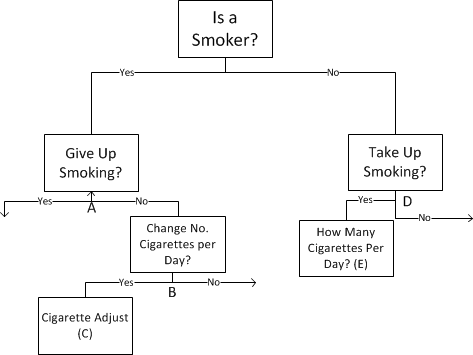
\includegraphics[scale=0.8]{DecTreeBasic2.png}
\end{center}
\caption{Initial Decision Tree}
\label{img:init-dectree}
\end{figure}

\begin{figure}
\begin{center}
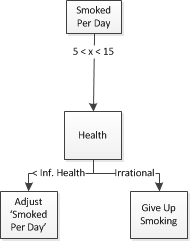
\includegraphics[scale=1]{example-decision.png}
\end{center}
\caption{Example Decision From Combination Decision}
\label{img:example-decision}
\end{figure}

\begin{landscape}
\begin{figure}
\begin{center}
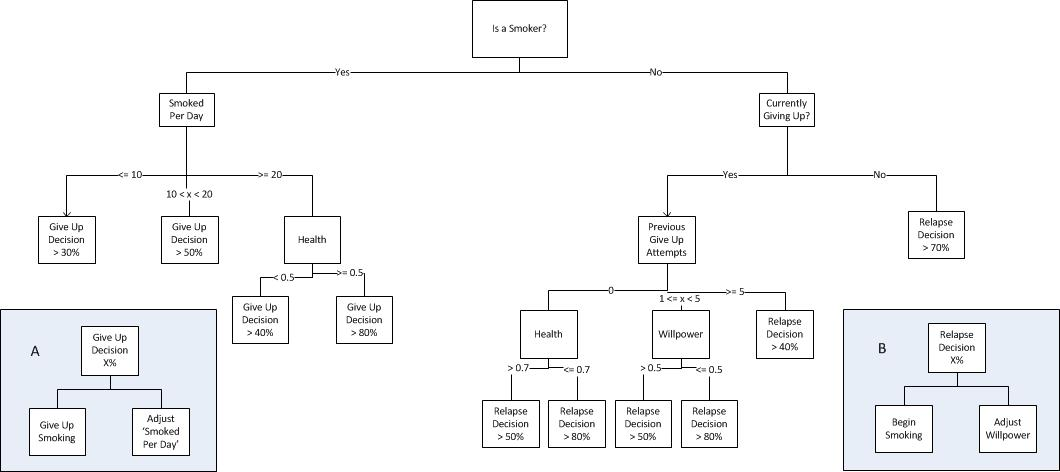
\includegraphics[width=\paperwidth,keepaspectratio]{DecTreev09.jpg}
\caption{Revised Decision Tree}
\end{center}
\label{img:0.9-dectree}
\end{figure}
\end{landscape}

\begin{figure}
\begin{center}
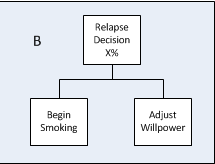
\includegraphics[scale=1]{End-DecA.png}
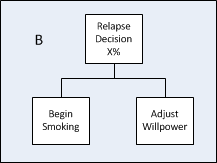
\includegraphics[scale=1]{End-DecB.png}
\end{center}
\caption{End Decisions in the Final Decision Tree}
\label{img:end-dec}
\end{figure}

\begin{figure}
Given a percentage threshold $p$, a node gives up if one or more of the below are true:
\begin{itemize}
\item $\text{influenced \% of neighbourhood giving up} > p$
\item $\text{\% non-smokers in neighbourhood} > 120\% \times p$ and $\text{random number} < \text{\emph{influenceability}}_{n}$
\item An irrational choice is made
\end{itemize}

Given a percentage threshold $p$, a node relapses if one or more of the below are true:
\begin{itemize}
\item $\text{influenced \% of neighbourhood smoke} > p$
\item $\text{random number} < \text{\emph{influenceability}}_{n}$
\item An irrational choice is made
\end{itemize}
\caption{Threshold Formulae for Decision Tree End Decisions}
\label{eq:end-thresh}
\end{figure}

During the course of development, simulations showed that some agents were on the borderline between smokers and non-smokers. This meant that they would switch between the two on a regular basis, potentially causing others in the neighbourhood to do the same. In an effort to avoid this, a measure was introduced that counts the number of turns since the last change and produces a probability, seen in equation \ref{eq:turns}, that slows down this rate of change by guarding the attribute swap from/to being a smoker with this probability against a uniform random number.

\begin{equation}
p(\text{\emph{change}}) = 1-\frac{1}{\text{turns since last change}\times 1000}
\label{eq:turns}
\end{equation}

For the `giving up' decision, labelled as \emph{A} in figure \ref{img:end-dec}, either the process of giving up begins (described in the attributes section above) or the number of cigarettes smoked per day is adjusted. The latter is done by comparing the influenced attribute value for cigarettes smoked per day against a percentage threshold. The threshold is a system parameter and creates a range around the agents own attribute. Should the influenced attribute be outside of this range, the agent has its attribute moved towards the influenced value by half of the influenced value, providing a gradual change. In terms of B, a small amount of willpower is removed should they relapse to smoking, otherwise it is added. These formulae can be see in figure \ref{eq:end-attr}
\begin{figure}
End Decision A - The value of $\text{\emph{smokedPerDay}}_{n}$ is changed for some node $n$:
\begin{itemize}
\item If a irrational choice is made or $\text{\emph{influenced smokedPerDay}}_{n} < \text{\emph{smokedPerDay}}_{n}\times\text{lower \% threshold}$, then $\text{\emph{smokedPerDay}}_{n} = \text{\emph{smokedPerDay}}_{n} - \frac{\text{\emph{influenced smokedPerDay}}_{n}}{2}$ 
\item If a irrational choice is made or $\text{\emph{influenced smokedPerDay}}_{n} > \text{\emph{smokedPerDay}}_{n}\times\text{upper \% threshold}$, then $\text{\emph{smokedPerDay}}_{n} = \text{\emph{smokedPerDay}}_{n} + \frac{\text{\emph{influenced smokedPerDay}}_{n}}{2}$
\end{itemize}
Where \emph{lower \% threshold} and \emph{upper \% threshold} are system parameters.\\

End Decision B - The value of $\text{\emph{willpower}}_{n}$ is changed for some node $n$:
\begin{itemize}
\item If $n$ relapses to smoking, and a $\text{random number} < \text{\emph{influenceability}}_{n}$ then $\text{\emph{willpower}}_{n} = \text{\emph{willpower}}_{n} - \text{\emph{willpower}}_{n}\times 0.001\%$
\item If $n$ remains a non-smoker, and a $\text{random number} < \text{\emph{influenceability}}_{n}$ then $\text{\emph{willpower}}_{n} = \text{\emph{willpower}}_{n} + \text{\emph{willpower}}_{n}\times 0.001\%$
\end{itemize}
\caption{Attribute Changes for Decision Tree End Decisions}
\label{eq:end-attr}
\end{figure}

Although this simplifies the decision-making process beyond that of human cognition, it allows a basic model of peer pressure and susceptibility to general influence. There is the potential for improvement through swapping this decision series with a more accurately modelled one would be straightforward. For the purposes of this model, it provides sufficient complexity and configurability since the thresholds can be set through the decision tree as part of the tuning process.
The final decision tree had a number of extra `decision layers' added to attempt a more accurate mapping of a real decision process; it can be seen in figures \ref{img:dectree-left} and \ref{img:dectree-right} with the initial decision that links the two in \ref{img:overarch}. The aim of this was to provide a more configurable and realistic decision-making model than the previous version, whilst keeping each attribute in a separate layer. Figure \ref{tab:attr-change} shows at which point in the tree any attributes are changed (outside of the end-states A and B), which are marked as \emph{ATTR}.


\begin{figure}
\begin{center}
\begin{tabular}{|l||l|p{10cm}|}
\hline
\bf{Label} & \bf{Attribute} & \bf{Change}\\
\hline
ATTR-1 	& \emph{health} 				&	$\text{\emph{health}}_{n} = \frac{\text{\emph{smokedPerDay}}_{n}}{\text{model cigarette limit} \times 1000}$, where the cigarette limit is a system parameter for the maximum number of cigarettes an agent can smoke per day		\\
ATTR-2	&	\emph{smokedPerDay}  	&	The same change as seen for end-decision A, seen in figure \ref{eq:end-attr}				\\
ATTR-3	&	\emph{health}					&	$\text{\emph{health}}_{n} = \frac{\text{\emph{stepsSinceGiveUp}}_{n}}{\text{giving up step limit} \times 1000}$, where the giving-up step limit is a system parameter for the number of steps before someone who is giving up is classed as a non-smoker \\
\hline

\end{tabular}
\end{center}
\caption{In-Tree Attribute Changes}
\label{tab:attr-change}
\end{figure}
For the currently `smoking' arm of the tree, a number of changes were made. The ability to give up in the `normal' smoker range (here 5 to 15 per day, but this could be adjusted) was only allowed by above average health. The rationale behind this is that whilst lighter smokers are likely to be more able to go without smoking~\cite{NHS-43}, gradually reducing their own consumption until they quit completely. On the other hand, heavy smokers are more likely to be strong in their resolve against giving up smoking, making their willpower an important decision factor compared to their health, due to the habit being harder to break. Health, however, is deemed more important for lighter smokers since any change in the number of cigarettes smoked may have more of an impact than for a heavy smoker. Furthermore, the fact that influenced health is used aims to represent how being less healthy than those in the neighbourhood would provide more encouragement of the person to attempt to give up, with the other side of this being that if someone smokes and is of above average health, they will not feel as much social pressure with regards to health.

For the non-smokers, the tree arm was also expanded to include new layers. If the agent hasn't failed at giving up before, then the willpower is considered most important as it represents their ability to continue the process of giving up. Health is included as a sub-point since if someone is healthier than their neighbours they might see that as a reason to continue their giving up effort. For those who have tried to give up a few times (between 1 and 5), the percentage of non-smokers/those giving up in the area dictates which route they should take, then leading into a decision based on willpower. The idea here is that since the agent has relapsed to smoking a number of times, the encouragement of the neighbourhood may have a greater effect on their own actions. In addition to this, the willpower decision is based on the influenced attribute for willpower, so the agent is effectively comparing their own resilience to those who surround them - if they are more resilient then it is assumed that they require more of their neighbours to be smoking to cause a relapse. If many (in this case more than 5) attempts at giving up have been made, a crowd mentality approach is used, where the giving up status of those around the agent dictates how susceptible they are to relapsing again. Influenced health is included since willpower appears to be irrelevant to these individuals; being more healthy than those in the neighbourhood leads to a lower chance of relapsing. Those who are not currently giving up are diverted to a more simplistic tree as they do not need their decision to be affected by how many times they have tried to quit before. Given that they have displayed the willpower to not smoke anyway, it is assumed that this is a less important factor than their health. In terms of health, the agent's own value is compared to the influenced attribute in an effort to model an attitude of health-awareness; if someone is of good health relative to others then they are less likely to risk it by smoking, whereas if they are of below average health, they may perceive smoking to make little difference.

The end-state decisions for each branch have a percentage threshold stated; the values shown on the diagram have been selected through a process of trial and error with the aim of providing as balanced a simulation as possible. Since some decision routes are more popular than others, the percentages need to account for this. With this in mind, they also represent the relative effect of that branch on the chance of giving up. An example is that if someone is a light smoker ($< 10$ cigarettes a day), has never tried to give up before and has higher than the influenced health, then it would be reasonable for them to be hard to convince to give up as they do not smoke a lot and are, compared to their social connections, quite healthy. To show this, that particular end-state requires more than 70\% of their neighbours to also be giving up before they will do the same.

In general, whilst this configuration of the decision tree was settled upon for performing simulations using the model, extra levels could easily be added or decisions rearranged. Ideally, this kind of decision-making process would be developed alongside in-depth psychological studies into the field so that an accurate and expansive tree can be built. Because this was beyond the scope of the project, an ad-hoc approach was used by designing the tree in accordance to model balance and real-life comparison, leading to assumptions about human behaviour having to be made.

\begin{figure}
\begin{center}
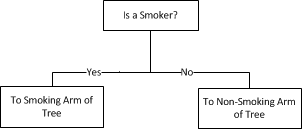
\includegraphics[scale=1]{overarch.png}
\caption{Overarching Decision Between the Smoking and Non-Smoking Arms of the Decision Tree}
\label{img:overarch}
\end{center}
\end{figure}

\begin{landscape}
\begin{figure}
\begin{center}
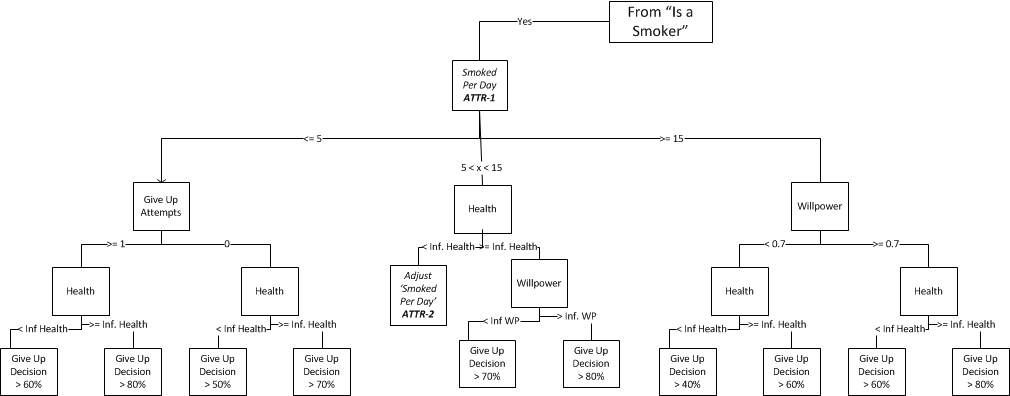
\includegraphics[width=\paperwidth,keepaspectratio]{Dectree-left.png}
\caption{Smoking Arm of the Final Decision Tree. Note that \emph{Inf} is influence and \emph{WP} is willpower.}
\label{img:dectree-left}
\end{center}
\end{figure}
\end{landscape}

\begin{landscape}
\begin{figure}
\begin{center}
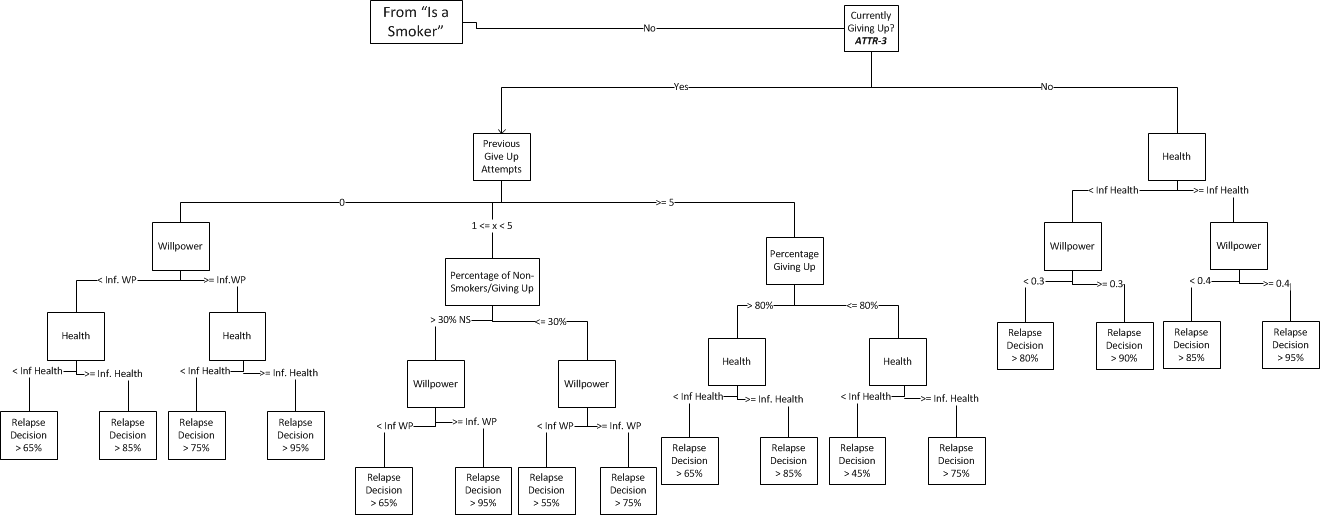
\includegraphics[width=\paperwidth,keepaspectratio]{dectree-right.png}
\caption{Non-Smoking Arm of the Final Decision Tree. Note that \emph{Inf} is influence and \emph{WP} is willpower.}
\label{img:dectree-right}
\end{center}
\end{figure}
\end{landscape}


\subsubsection{Connection Reconfiguration Actions}

The final stage of the agent actions is to reconfigure their connections to the neighbourhood. By this point, the agent has assessed the neighbourhood and made changes to their attributes where appropriate, so based on this new information the agent can now look to remove any relationships to others who are now too dissimilar or for new agents that are closer to their personalities. From the initial research, the concept of homophily emphasises the importance of this likeness so to emulate this, the chosen method of comparing agents was to generate a scoring algorithm, seen in figure \ref{code:scoring}. This way, any two agents could be compared at any point and a valur to represent their similarity produced.

Different attributes have different weightings when it comes to comparing agents. As the algorithm is intended to imitate the process of a human looking to their circle of connections for  similar people, someones \emph{influenceability} is likely to have less impact than whether they have the same smoking behaviours, for example. To account for this, the scoring algorithm uses different score values for each attribute which can be seen in figure \ref{tab:reconfig}. Another factor in the weighting is that of how the difference is used in scoring. The algorithm offers three options, the formulas for which can be seen in figure \ref{code:comp-methods}: \emph{percentage difference}, \emph{attribute comparison} and \emph{linear scoring}.

\emph{Percentage difference} is most commonly used since it provides a scaled score within a range of $\pm50\%$ of the current agents attribute score. This means slightly different things for different attributes but in general, the higher scoring someone is in an attribute, the more accepting they are of others; an example might be that light smokers would consider someone who smokes a few more cigarettes a day more to be of similar difference to themselves as a heavy smoker would to someone who smokes half their intake. \emph{Attribute comparison} is a more straightforward mechanism, simply giving an amount of points should two attributes be the same, or in the case of \emph{stepsSinceGiveUp}, below a certain value. Finally, \emph{linear scoring} is only used by \emph{influenceability} and is a way to incorporate the susceptibility of someone to peer pressure into the score. No scoring is done against the other agent for linear scoring, since it is based on the attributes of the current agent only. A disadvantage of this method is that it greatly simplifies what humans might look for in social ties as it assumes that they are only interested in those who behave similarly. Although this is not the case in reality though for the sake of avoiding modelling this connection seeking in a high level of detail, which would take a lot of time, the assumption will stand for the project. If required, the scoring method could be substituted for one which accounts for one which handles the interplay of personality in a more detailed manner.

\begin{figure}
\begin{center}

\begin{tabular}{|l||l|l|l|}
\hline
\bf{Attribute} & \bf{Minimum Score} & \bf{Maximum Score}\\
\hline
\emph{isSmoker} 						& 0	&	1\\
\emph{givingUp}						&	0	&	2\\
\emph{health}							&	0	& 5\\
\emph{willpower}						&	0	&	5\\
\emph{sociable}						&	0	&	2\\
\emph{influenceability}		&	0	&	3\\
\emph{stepsSinceGiveUp}		&	0	&	5\\
\emph{smokedPerDay}				&	0	&	5\\

\hline

\end{tabular}
\end{center}
\caption{Scoring Algorithm Upper and Lower Bounds for Scores}
\label{tab:reconfig}
\end{figure}

\begin{figure}
\begin{center}
	\begin{lstlisting}
for(Node n : Neighbours)
{
	//Attribute comparison
	if(current.isSmoker == n.isSmoker)
	{
		score + 1
		//Attribute comparison
		if(current.isGivingUp && n.isGivingUp)
		{
			score + 2
			//Attribute comparison score
			if(n.stepsSinceGiveUp less than 1.5 times 
				current.stepsSinceGiveUp)
				score + 5
			else
				score + 2
		}
		//Attribute comparison
		if(current.isSmoker)
		{
			score + percentScore(smokedPerDay) 
		}
	}
	score + percentScore(health)
	score + percentScore(willpower)
	score + percentScore(sociable)

	score + linearScore(influenceability)

	return score/28
}
	\end{lstlisting}
\end{center}

\caption{Scoring Algorithm Pseudocode}
\label{code:scoring}
\end{figure}

\begin{figure}

\begin{itemize}
\item \emph{Linear Scoring} - The attribute is multiplied by the maximum s
\item \emph{Percentage Scoring} - The percentage difference between attributes is calculated ($\frac{\text{attr}_{this}-\text{attr}_{other}}{\text{attr}_{other}}$). If they are separated by more than 100\%, the minimum score is given, otherwise $\text{\emph{score}} = \text{\emph{maximum score}} - \text{\emph{\% difference}} \times \text{\emph{maximum score}}$.
\item \emph{Attribute Comparison} - Two values are compared and if they are the same (or within some defined range), the maximum score is given, otherwise a lesser score is given.
\end{itemize}
\caption{Comparison Methods Between Agents}
\label{code:comp-methods}
\end{figure}

Once a score has been calculated and normalised to between 0 and 1, this can be used to determine if the two agents should form a connection, remove an existing one or do nothing. The method for this is to have two simulation parameters, \emph{ConnectionScoreRemoveBound} and \emph{ConnectionScoreAddBound}, which dictate the boundaries for action to be taken. The `remove boundary’ must be lower than the `add boundary’ and if the score is below the former boundary, the edge is removed. Should the agent score be above the add boundary, then the edge between the agents is added. New edges have their influence set through a normal distribution with a mean of their normalised similarity score, minus 0.5 to a more central position rather than the generally higher value that would be given otherwise. This is because a high score is required to connect to begin with, so all new edges would be of influences higher than the `add boundary'. Experimentation has shown this to give a more reasonable distribution of influences.

It should be noted that as part of the effort to keep the model balanced, limits were imposed on the number of connections that each node can have. Should another edge be added when the node has reached its limit, the lowest influence edge is removed in favour of the new connection. Once again, the limit a simulation parameter so can be changed to investigate the effects that is has, though testing indicated that it mainly helped avoid clustering and excessive connection-forming with other nodes. Especially important in this area are the boundary values. By lowering the upper bound to 0.6, the graph significantly increased its chance to become very dense and turn into a tight cluster  (figure \ref{img:ex-crunch}), whereas a raising it to 0.7 maintained a much better balance and avoided the clustering, as seen in figure \ref{img:ex-noncrunch}, whilst the removal boundary was kept at 0.4.

Finally, in order to introduce external influences to a neighbourhood, every agent has a small chance to form a random connection to some other agent in the graph. This is deliberately set to have a very low occurrence rate as testing showed that setting the probability to be any more than 0.002\% of \emph{sociability} lead to regular addition of edges, effectively rendering the scoring algorithm useless and resulting in an incredibly dense graph. By making this a rare event, it attempts to model the day-to-day chance of a new influence entering a humans life i.e. meeting a new person or taking on a new role-model. Over the course of the simulation, there is a chance that nodes may become disconnected from others. As it is unrealistic for humans to have absolutely no social connections, the model reconnects them to a random node in the network with a 30\% chance of connection. This is not a certain reconnection since to reach a disconnected state, the edge must have held attributes such that it fell below the removal boundary of its neighbour nodes; by doing this, it gives the node a chance to connect and move to a new area of the network.

% --------------------------------
%
%		END OF IMPLEMENTATION
%
% --------------------------------

% --------------------------------
%
%			  RESULTS
%
% --------------------------------
\chapter{Simulation Results \& Model Analysis}
\label{sec:analysis}
\section{Overview}

To understand whether the developed model provides useful results and meets the initial specification, two separate methods were used. Firstly, the model was used to run simulations, providing a number of pieces of information for analysis. In regards to the problem domain, finding out new information about the impact of social networking upon smoking is a key aim, but at the same time, these simulations should help to demonstrate whether the model is balanced, efficient and a good base for future work. Following this, analysis of the model from a qualitative viewpoint will form the second part of this section. As a part of the specification concerns itself with understanding whether the model is a suitable proof-of-concept for a commercial model, this is combined with general thoughts on the quality of the model and any future improvements. The basis of this analysis comes from both the design decisions and the results of the simulations carried out.

\section{Simulation Analysis}
Using the developed model, a wide range of possible situations can be simulated through using generated or sampled graphs along with configuring certain percentages of the population to smoke, give up or not smoke at all. Whilst running all of these simulations is beyond the scope of this project, ones displaying promise of interesting results were run instead. Two main categories chosen: \emph{simulation parameters} and \emph{sampled networks}.

For all simulations, 30,000 simulation steps were carried out with graph and attribute files being exported every 1000 steps. A simulation step is a difficult concept to assign a unit of time to since it is discrete and involves making decisions, assessing influence and rearranging social ties all in one movement. In light of this, the simulation length, whilst not given a specific time period, should be considered to represent months and days rather than hours.

\subsection{Simulation Parameters \& Agent Attributes}

Given the number of agent attributes and system parameters, there are many initial configurations to sumlate. Since some of these do not map to real-world concepts in the problem domain, they were not be covered in favour of those with a more direct connection. To begin with, a high-level investigation into the percentage split of smokers and non-smokers in the starting state was conducted using a base graph as seen in figure \ref{img:simbase}. The aim of this test was to get a better understanding of how starting combinations of the graph, relative to percentages of smokers and non-smokers, related to the number of non-smokers left at end of the simulation. Simulations were run for smoking percentages of 20\% to 80\%, in intervals of 20\% whilst within these groups, the percentage of the non-smokers giving up was varied from around 10\% to 80\% over five runs. The results can be seen in table \ref{tab:stats}; note that the values are not exactly on the percentage boundaries as attribute assignment is probablistic.

%A number of runs were executed with the results visible in FIG Y.

\begin{figure}
\begin{center}
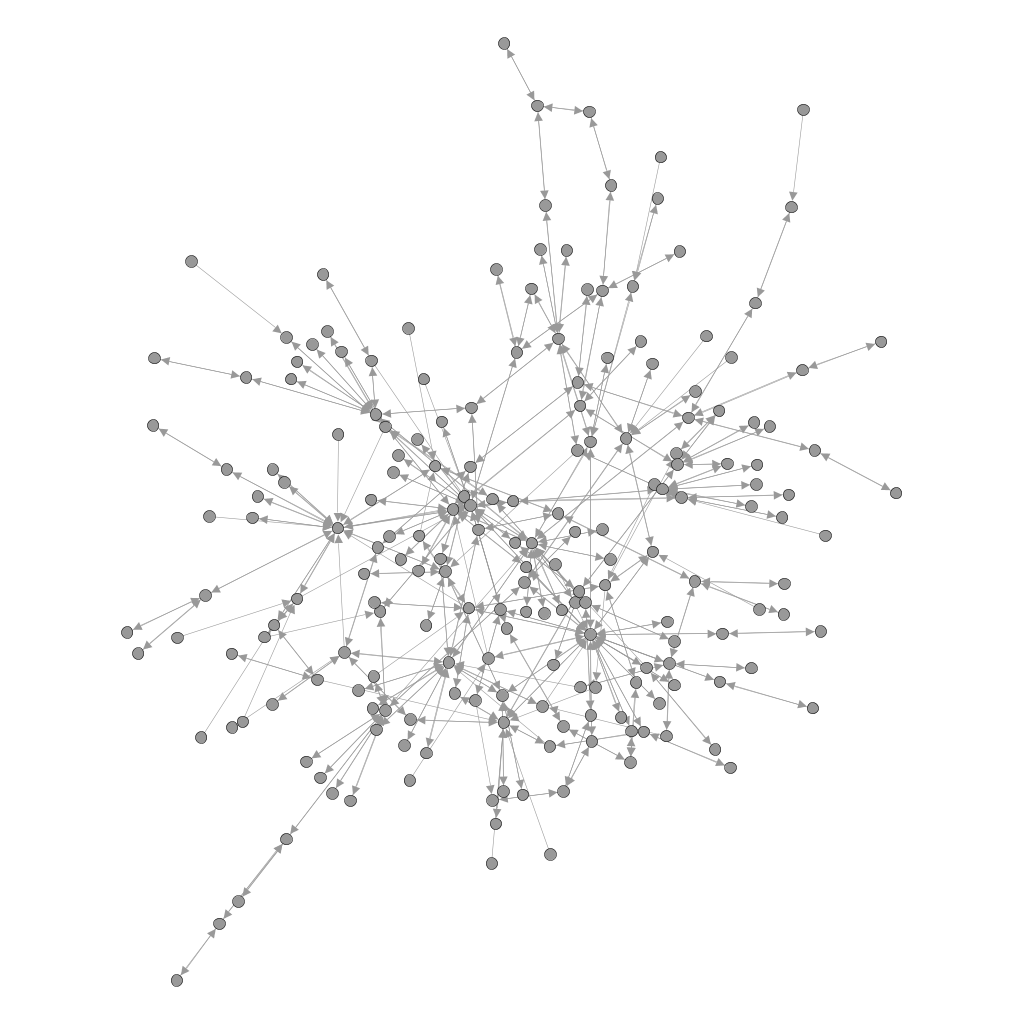
\includegraphics[scale=0.5]{simbase.png}
\end{center}
\caption{Simulation Base Graph}
\label{img:simbase}
\end{figure}

\begin{landscape}
\begin{figure}
\begin{center}
\begin{tabular}{|c|c|c|c|c|c|c|c|}
\hline
\multicolumn{4}{|c|}{\textbf{Starting Split (\%)}} & \multicolumn{4}{|c|}{\textbf{Ending Split(\%)}}\\
\hline
Smoking & Giving Up & Non-Smoking & Non-Smoking/Giving Up & Smoking & Giving Up & Non-Smoking & Non-Smoking/Giving Up\\
\hline
19.4 & 	8.7	 &	71.9 &	80.6 &	45		&0		&55	 &	55		\\
23.5 & 	25	 &	51.5 &	76.5 &	25.5	&0.5	&74	 &	74.5		\\
20.4 &	34.7 &	44.9 &	79.6 &	25		&0		&75	 &	75		\\
20.9 &	54.1 &	25	 &	79.1 &	26.5	&0		&73.5 &	73.5	\\
17.3 &	63.8 &	18.9 &	82.7 &	26.5	&0		&73.5 &	73.5	\\
23	 &	77	 &	0	 &	77	 &	26.5	&0		&73.5 &	73.5	\\
\hline
42.3 &	8.7	 &	51	 &	59.7 &	34.1	&0		&65.9 &	65.9	\\
40.3 &	16.8 &	35.3 &	52.1 &	52		&0		&48	 &	48		\\
47.9 &	23.5 &	28.6 &	52.1 &	50.5	&0		&49.5 &	49.5	\\
36.7 &	42.3 &	21	 &	63.3 &	31.6	&0		&68.4 &	68.4	\\
44.9 &	45.4 &	9.7	 &	55.1 &	31.2	&0		&68.8 &	68.8	\\
38.3 &	61.7 &	0	 &	61.7 &	33.6	&0		&66.4 &	66.4	\\
\hline
59.7 &	8.1	 &	32.2 &	40.3 &	18.9	&0		&81.1 &	81.1	\\
58.2 &	13.3 &	28.5 &	41.8 &	36.7	&0		&63.3 &	63.3	\\
61.7 &	15.3 &	23	 &	38.3 &	12.8	&0		&87.2 &	87.2	\\
53.6 &	29.6 &	16.8 &	46.4 &	20.9	&0		&79.1 &	79.1	\\
60.2 &	29.6 &	10.2 &	39.8 &	45		&0		&55	 &	55		\\
56.6 &	43.4 &	0	 &	43.4 &	45		&0		&55	 &	55		\\
\hline
80	 &	3	 &	17	 &	20	 &	31.6	&0		&68.4 &	68.4	\\
77.5 &	7.14 &	15.36 &	22.5 &	56.7	&0		&43.3 &	43.3	\\
77.6 &	9.7	 &	12.7 &	22.4 &	36.7	&1.5	&61.8 &	63.3	\\
79.1 &	13.8 &	7.1	 &	20.9 &	68.9	&0		&31.1 &	31.1	\\
78.1 &	17.3 &	4.6	 &	21.9 &	27		&0		&73	 &	73		\\
77.6 &	22.4 &	0	 &	22.4 &	23.5	&0		&76.5 &	76.5	\\

\hline
\end{tabular}
\end{center}
\caption{Percentage Split of Smokers and Non-Smokers at the Start and End of Simulations. Ordered by Starting Smoking \% Split.}
\label{tab:stats}
\end{figure}
\end{landscape}

From figure \ref{img:smok-give}, it can be seen that as the ratio of those giving up compared to those smoking at the start of the simulation increases, the final percentage of those who do not smoke at the end becomes much more unpredictable. One possible explanation for this is that these people, since they have already given up once, will find it easier to relapse to smoking; if many people start to do this, the influence may then persuade others to do the same causing the final split of smokers and non-smokers to be largely dependent on how connections have formed over the earlier stages of the simulations. Continuing from this, figure \ref{img:smok-pct} shows the percentage of smokers in the network at the start against those who are not smoking at the end. For lower starting percentages of smoking such as 20\%, the percentage not smoking at the end is around 70\%, which is as expected from a stable simulation. When the percentage of smokers increases, the range of ending percentages also increases to the point where at 80\% being to start, the quantity giving up at the end is between 30\% and 75\% of the graph. This points to the possible effect of a core of people giving up having an effect on the smoking population - at low percentages of smokers, those giving up are less likely to interact with smokers so have a lower chance of influencing them. For higher starting smoker percentages, the people giving up are much more likely to be surrounded by smokers and as such be affected by the influence. As described above, the impact of this influence largely depends on how the network has changed since in the case where around 80\% of the graph start as smokers and the ends at with 75\% not smoking, wide-spread cessation occurred. On another run with the same starting smoker percentage but different amount giving up (22\%), significantly fewer were non-smokers at the end.

Whilst there is no clear conclusion from these tests in regards to the optimal situation for giving up, it does provide insight into the model itself. It appears that having a larger proportion of those giving up or not smoking as part of the network to begin with destabilises the results somewhat. It indicates that, due to the higher quantity of smokers surrounding those giving up or not smoking, relapses are more common. Additionally, a high percentage of smokers takes a longer time to persuade to give up via influence. As a result, it may be the case that agents attempt but fail to give up smoking regularly, never providing a constant source of influence to others but instead dissipating inconsistent influence to others. This inconsistency then can spread throughout the network to others who are trying to give up and given that there is a larger portion of the network able to do this when the majority of the graph smokers, this could explain the unpredictability in the above results. In regards to real-world behaviour, the main discovery is that trying to get networks saturated with smokers to give up is very difficult and simply introducing some non-smokers is not enough. Instead, it would seem that the optimal way for this to be tackled is that large chunks of the network would need to give up simultaneously, driving down the percentage of smokers overall.

\begin{figure}
\begin{center}
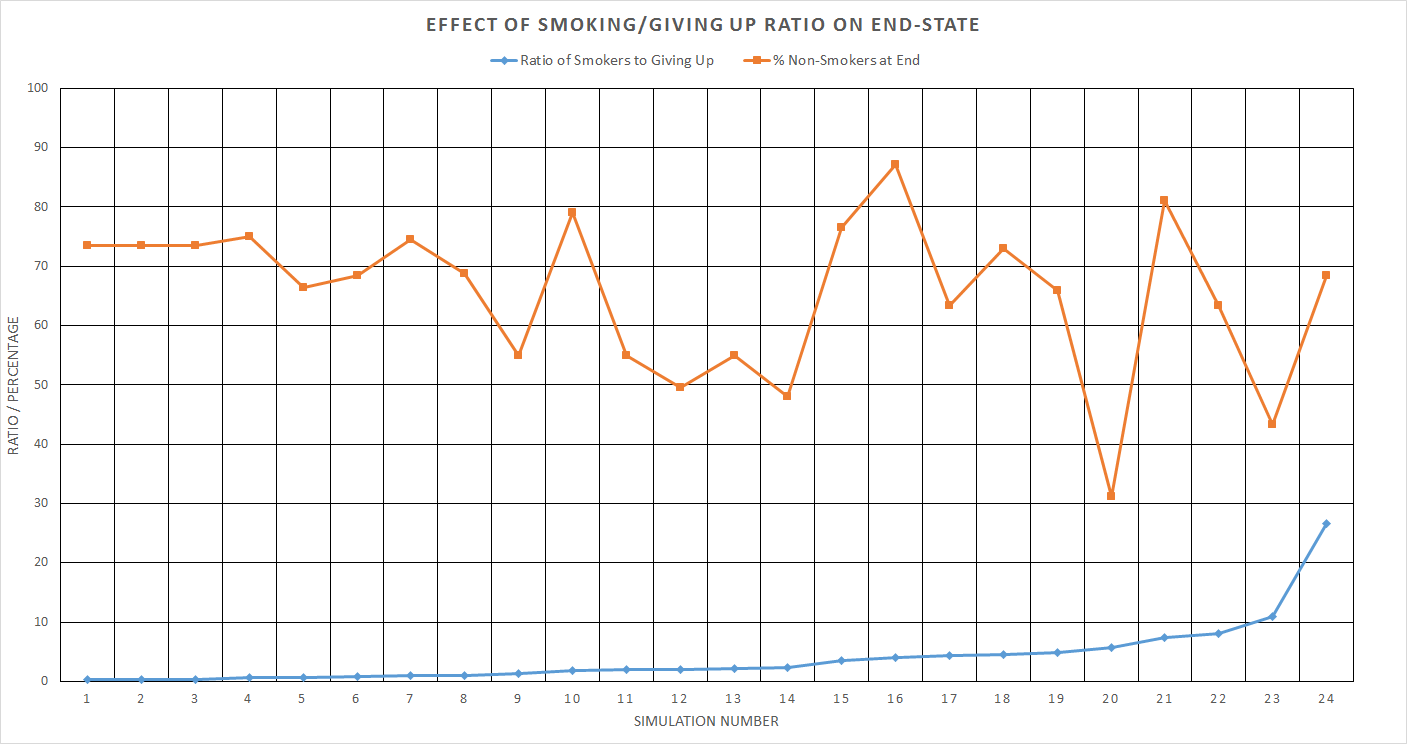
\includegraphics[width=\textwidth]{smok-giveup.png}
\end{center}
\caption{A comparison of the ratio between the percentage of smokers and those giving up at the start of the simulation against the percentage of non-smokers (including those giving up) at the end.}
\label{img:smok-give}
\end{figure}

\begin{figure}
\begin{center}
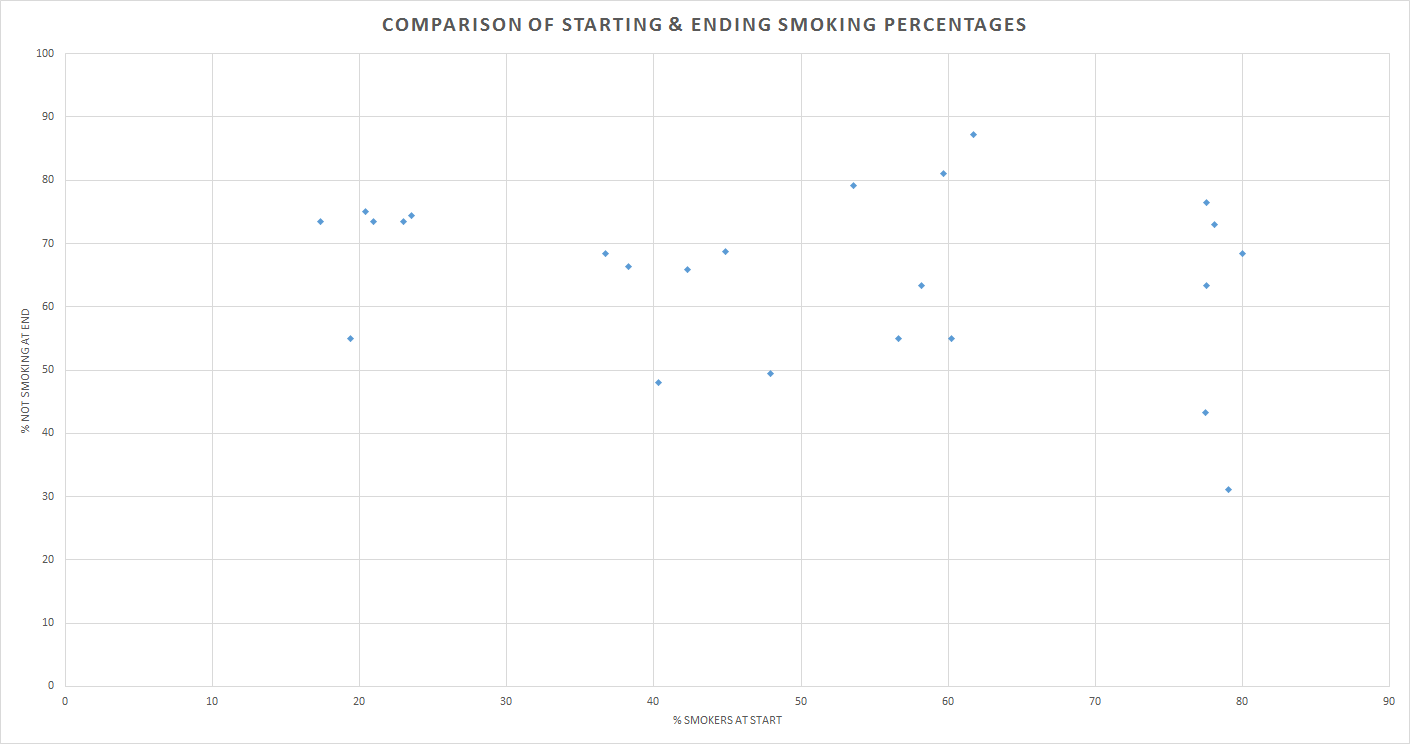
\includegraphics[width=\textwidth]{smok-pct.png}
\end{center}
\caption{A comparison of starting percentage of smokers in the graph and the ending percentage of non-smokers.}
\label{img:smok-pct}
\end{figure}

In terms of other parameters that affect simulation results, the period of time taken before someone who is `giving up' becomes a complete non-smoker displayed an interesting trend. By varying the number of simulation steps required for this change, values between 750 and 1250 displayed an 86-94\% non-smoker finish percentage for a graph starting with 50\% non-smokers (of which 25\% are giving up) which is shown by the dip in the graph in figure \ref{img:give-up}. Compared to the other values tested, which produced non-smoking end figures of around 60-70\%, this is a significant drop. Should this be mapped to a more realistic scenario, it could imply that subjecting those who are giving up to pressure to maintain this for extended periods of time can actually have a negative effect but at the same time, allowing those who have only given up for a short time to consider themselves non-smokers can lead to many failed attempts, resulting in more smokers overall.

\begin{figure}
\begin{center}
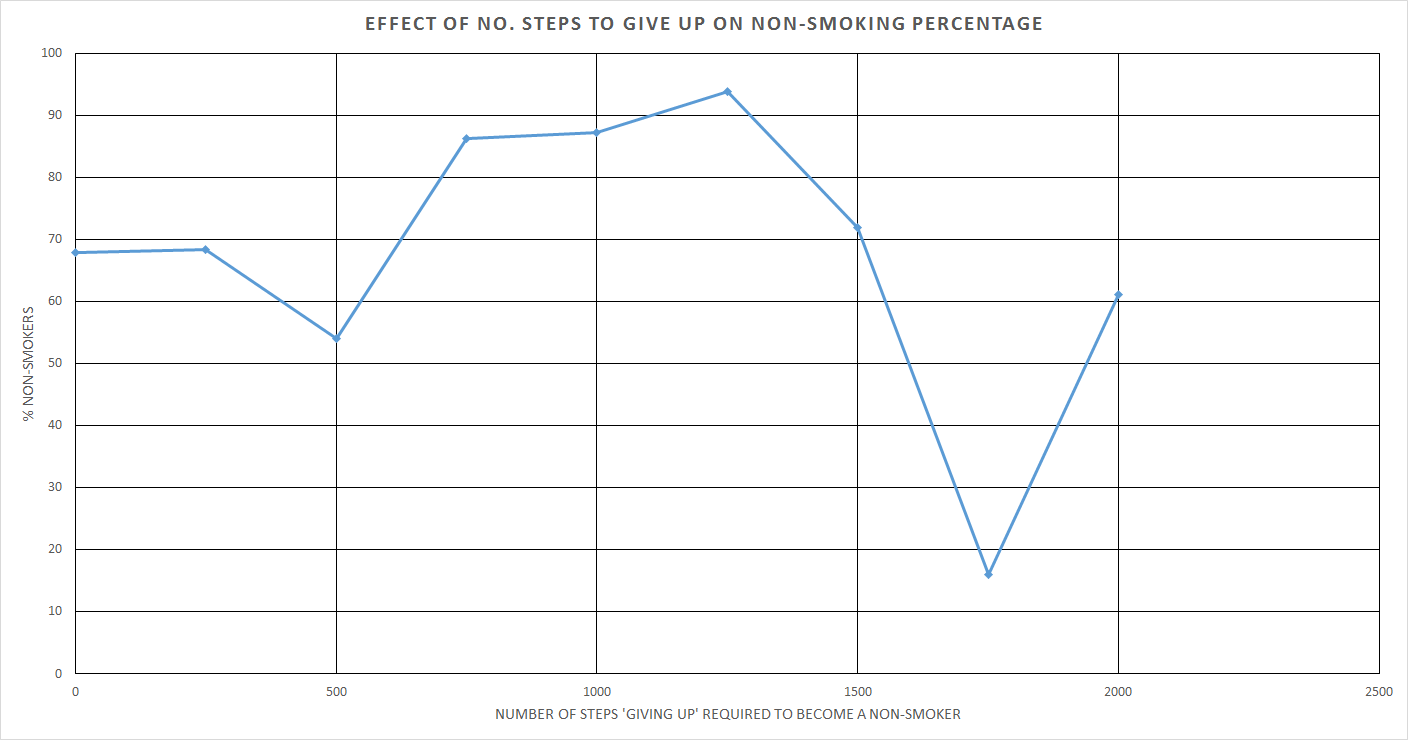
\includegraphics[width=\textwidth]{give-up.png}
\end{center}
\caption{The effect of the number of steps required for an agent to `give up' for before they become a non-smoker who is not giving up.}
\label{img:give-up}
\end{figure}

Another parameter which appeared to change the results of simulations was that of the mean value used to distribute the number of cigarettes smoked per day. As the graph in figure \ref{img:mean-cig} shows, increasing the value up to around 25 cigarettes per day causes the number of non-smokers in the network by the end of the simulation to peak at around 95\%. Since this is the value used to base the normal distribution of the cigarettes smoked per day at the start of the simulation, this result indicates that when heavier smoking is the norm, more of these smokers tend to quit. This could be due to a `group quit' as the group gradually lowers the number of cigarettes until they quit though in general, this result is not as predicted. As described in decision tree description (Section \ref{sec:dectree}), it was presumed that those of lower cigarette consumption would be more likely to cease smoking. It is definitely the case, however, that the majority of smokers would, at the start of the simulation, pass through the section of the decision tree for heavy smokers (seen in figure \ref{img:dectree-left}), where if they are of low willpower and lower than average health, they will stand a good chance of giving up. In regards to this being related to a realistic situation, it might be the case that lighter smokers see less of an effect on their health and if they are surrounded by those of similar consumption, they will be less likely to quit. Heavy smokers, on the other hand, notice more of a health effect and as such are more likely to give up.

\begin{figure}
\begin{center}
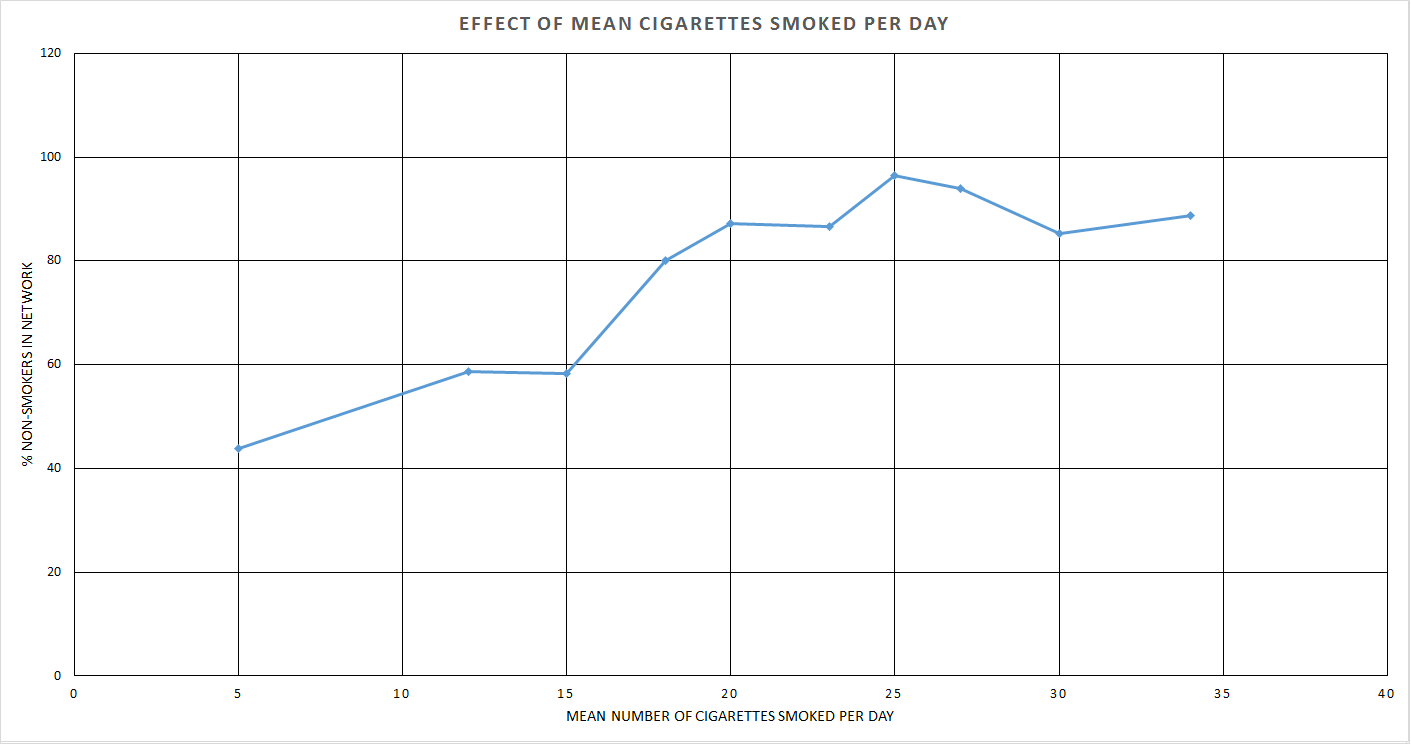
\includegraphics[width=\textwidth]{mean-cig.png}
\end{center}
\caption{The effect of the mean number of cigarettes smoked per day at the start of the simulation on the percentage of non-smokers at the end.}
\label{img:mean-cig}
\end{figure}


\subsection{Decision Tree Analysis}
As the decision tree is the major factor in selecting the behaviours of agents, the number of `hits' upon each decision reveals a lot about how individuals are guided to their final choice. To get a dataset for this, a scale-free graph with 483 nodes, 20\% being smokers and 10\% of the non-smokers giving up in order to be close to the UK smoking statistics~\cite{NHS-12}~\cite{NHS-43}, was simulated over a period of 30000 steps with every decision made by an agent being recorded. The final percentage of smokers was around 9\%, a moderate decrease in quantity but by no means significant due to the ratio of smokers to non-smokers. Figures \ref{img:dectree-right-lab} and \ref{img:dectree-left-lab}  shows the decision tree labelled with both the percentage of total `hits' and the percentage share of hits for the parent decision.

\begin{landscape}
\begin{figure}
\begin{center}
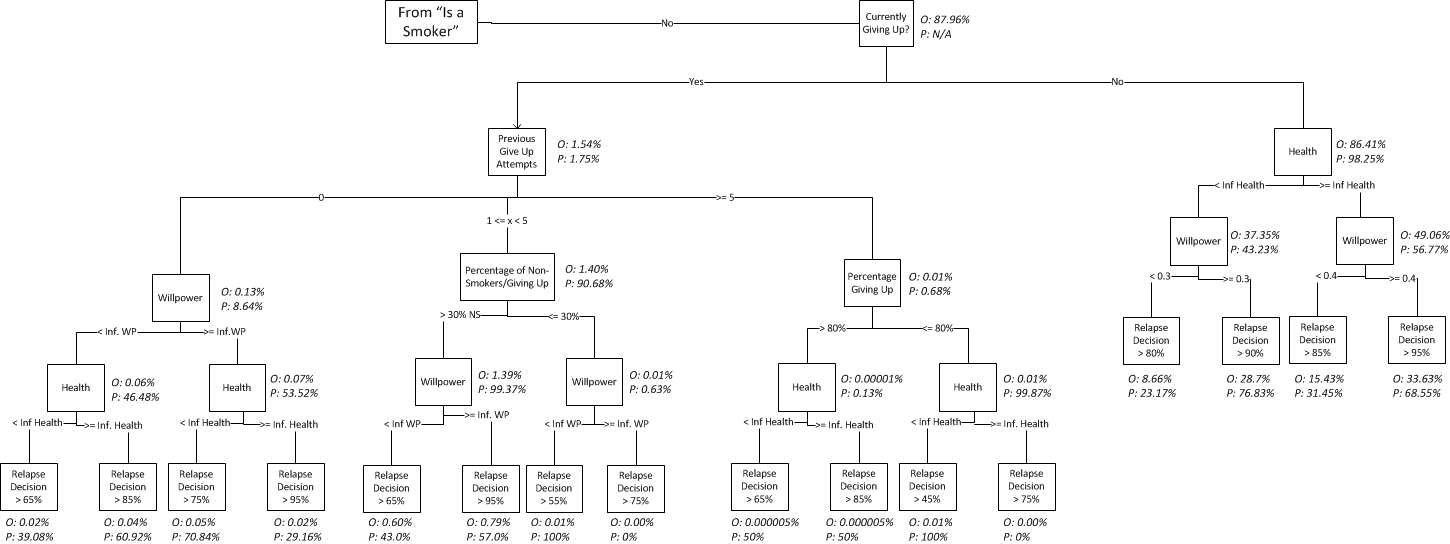
\includegraphics[width=\paperwidth,keepaspectratio]{dectree-right-labelled.png}
\caption{Non-Smoking Arm of the Final Decision Tree. Labelled to indicate flow of decisions, where O is the percentage of all decisions and P is the percentage of the decision from its parent.}
\end{center}
\label{img:dectree-right-lab}
\end{figure}
\end{landscape}

\begin{landscape}
\begin{figure}
\begin{center}
\includegraphics[width=\paperwidth,keepaspectratio]{dectree-left-label.png}
\caption{Smoking Arm of the Final Decision Tree. Labelled to indicate flow of decisions, where O is the percentage of all decisions and P is the percentage of the decision from its parent.}
\end{center}
\label{img:dectree-left-lab}
\end{figure}
\end{landscape}

In regards to overall percentage share of hits, the values appear as expected; the `non-smoking' arm of the tree encounters more hits than the smoking arm since a greater portion of the network does not smoke than does. Within the smoking arm, 70\% of agents fall in the middle branch, i.e. the `moderate' smoker, meaning that they do not have a high chance of giving up. Furthermore, 20\% of agent hits were to the `heavy' category, where although they do have a direct chance of quitting, it is unlikely due to the attributes used in that sub-tree, e.g. willpower. From this it may be deduced that to get a greater proportion of these smokers to try to give up they would need to be surrounded by people who smoke less than they do so that their influenced attribute for the quantity of cigarettes smoked would decrease. In turn, this would let them fall into the `light' smoker category which has a higher chance of giving up. Another explanation for the underrepresented section of light smokers is that few hit this decision regularly because instead, they give up smoking. Interestingly, if the end-states of the light smoker sub-tree are considered, both choices left a greater proportion of the agents going to the option which required a higher local percentage of non-smokers to give up, which implies that there is a core of light smokers who do not give up. To have the previously described scenario of lighter smokers encouraging heavier ones to reduce consumption, a greater percentage of lighter smokers would be required over the course of the simulation whilst avoiding having so many that it would skew the tree, making it too difficult to give up because of a high percentage of smokers being in the graph.

Of the medium and heavy smoker groups, looking at deeper levels of the tree points to areas which could be targeted to encourage cessation. For the former group, the majority of hits was traced to the agent reassessing their smoking consumption, with the majority of this sub-group opting to reduce consumption. Some, however, were given the chance to quit with the larger portion taking the marginally easier route of 70\% of the neighbourhood needing to be not smoking. This matches with the above idea of getting smokers down to lower consumptions before giving up, which could again be improved by planting more, high influence, low consumption smokers in the area. For the `heavy' smokers, there is a fairly even split across all sub-groups. It should be noted that there is an `easy' chance for heavier smokers to give up if their health is lower than those they are related to, though this was not any more popular than any of the other decision routes. This indicates that to get this group to stand more chance of quitting, they would need to be surrounded by people who smoke either less than they do or not at all, and also are of better health. Doing this would guide them to either the light smoker options or the 'easy' option within the heavy smoker tree - one which requires both low health and willpower.

For non-smokers, it is most important to direct them away from end-states where there is a chance to either begin smoking or relapse whilst giving up. Groups of agents giving up mainly visited the branch for those who have tried to give up between 1 and 5 times. As a side note, this is encouraging for the model balance as it shows that the majority of individuals do not fall into a cycle of giving up and relapsing which would be alluded to by a lack of hits in this area but many for either no previous or more than five attempts. Within this group, the vast majority had more than 30\% of their neighbours as non-smokers so had a lower chance of relapsing. Due to the fact that willpower was the next factor to decide upon, there was a mostly even split since this attribute appeared to be evenly distributed. This is the key part of the branch since it shows that by having a contingent of not only non-smokers, but also agents of lower willpower with high influence will lead to the individual finding it easier to avoid smoking again. The section of agents with more than 5 attempts at giving up needed to be surrounded by others giving up - intended to emulate the effect of group support to those who have failed multiple times before - but were often not, meaning that they had a higher chance of relapsing. In the simulation it can be seen that all of the agents had lower than the influenced attribute for health, so stood a much higher relapse chance. To avoid this situation, individuals who have failed multiple times before need to be surrounded by a high quantity of others also giving up, ideally of similar health to their own to reduce their chance of relapse. The final section of the `giving up' sub-tree is that of the people with only one giving up attempt. Although most agents were of willpower higher than the threshold, the split in health reveals that to increase their chances of not beginning smoking, others of similar or lower health need to be in their neighbourhood. This also holds true for those of lower willpower.

The final section of the tree is that of non-smokers who are not currently giving up. As implied by the final smoker/non-smoker percentage split, the majority of the decision hits of the graph were in this area. On the next layer of the tree, a slight skew is present towards the agents being of higher than their influenced health, however to maintain a higher chance of avoiding smoking it must be ensured that the agent is surrounded by people of similar health. At the next decision down, willpower is used; a higher willpower here results in a lower chance of relapsing. Since this is not affected by the willpower of those in the neighbourhood (i.e. influenced willpower is not used), the most important decision here is on the previous level, which is that of the health. To be more specific, those of low willpower should be in a neighbourhood of lower health but high influence agents, whereas higher willpower individuals can afford to be around those of similar or higher health.

In general, the decision tree reveals a number of pointers for how to drive the network in the direction of giving up smoking then avoiding relapsing. Having smokers convinced to either smoke less per day or be surrounded by healthy, non-smokers helps in getting them to quit whilst positioning those who are giving up in the correct neighbourhood has a large effect on their chance of relapse with the exact composition of this neighbourhood depending on how many times the person has tried to quit before. From a model-focussed perspective, the above results indicate how important social ties are to the agents, as many decisions are based on the input of the neighbourhood.

\subsection{Sampled Networks}
In order to consider how the model functions with real networks, an example dataset was sampled. This is from the \textbf{Stanford SNAP}~\cite{SNAP} which provides a number of large datasets sampled from various internet sources. To maintain consistency with the system as a whole, only directed non-multi-graphs were used; undirected graphs would lack the required level relationship information whilst multi-graphs could have many of the same edge which is not catered for in this model. Generally, these datasets were very large and due the timescale of the project, the simulations could not take place on a cluster or HPC so instead a sample using the previously mentioned snowball sampler was taken and simulations run upon it. The simulation ran for 30,000 steps.

The dataset was of an email network~\cite{SNAP-email}, with the starting and ending states shown in figures \ref{img:sample-init} and \ref{img:sample-fin}. It was started with 50\% of the network smoking and of those not smoking, 50\% giving up, whereas by the end 80\% of the network were non-smokers. Over the course of the simulation, the average degree of the graph increased slightly from 2.198 to 2.431 with the network diameter decreasing from 34 to 25 and the average clustering coefficient going from 0.02 to 0.009. Although the connectivity of the graph increased, with both degree increasing and diameter decreasing, the average path length increased from 8.998 to 9.372. Generally, this implies that the graph has become slightly more disconnected over the course of the simulation which is not as expected since the reconfiguration by the agents should be balanced and should not remove too many edges, though this case was not too extreme. Ideally, higher connectivity would be achieved as it allows a greater spread of influence. This is illustrated by the contraction of the graph - the nodes in figure \ref{img:sample-init} are more spaced than in figure \ref{img:sample-fin}.

\begin{figure}
\begin{center}
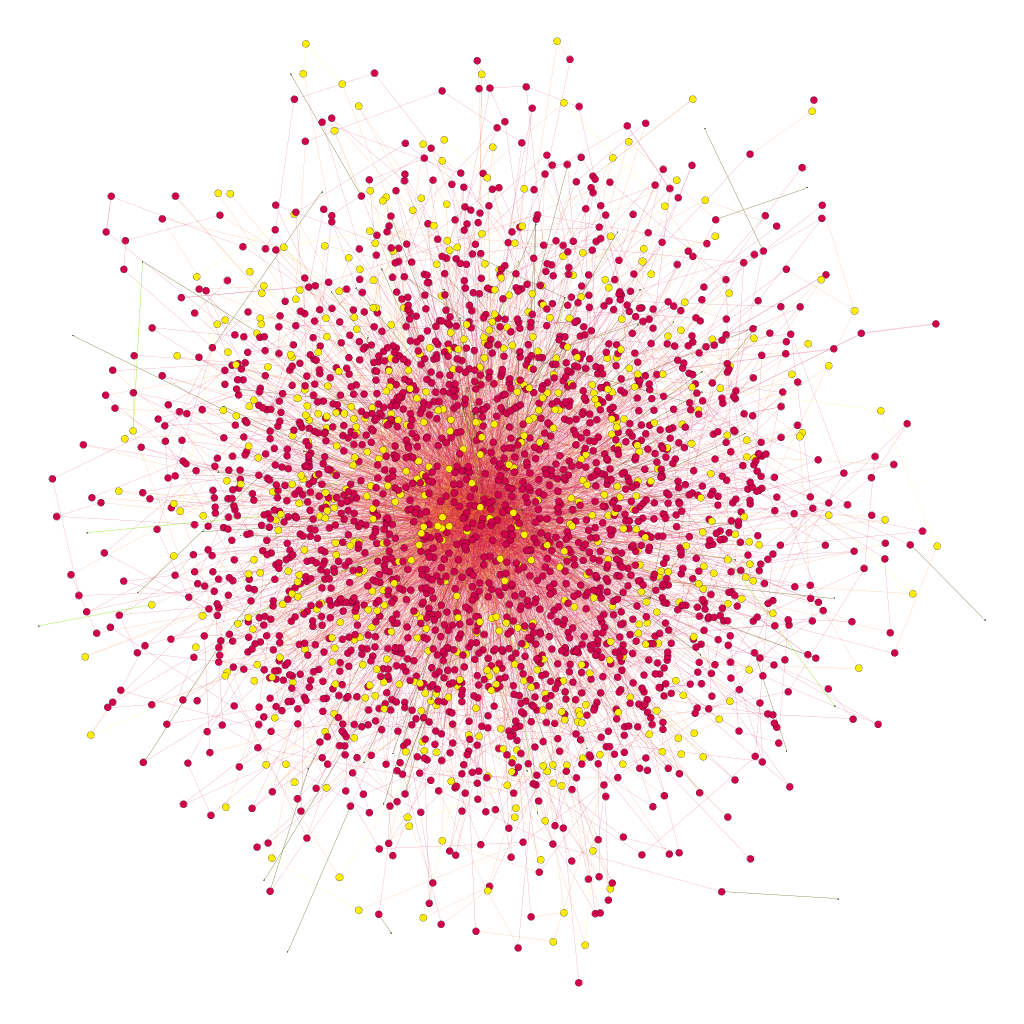
\includegraphics[scale=0.4]{sample-init.png}
\end{center}
\caption{Sampled network at the start of the simulation. Note that lighter nodes are smokers, whereas darker ones are non-smokers.}
\label{img:sample-init}
\end{figure}

\begin{figure}
\begin{center}
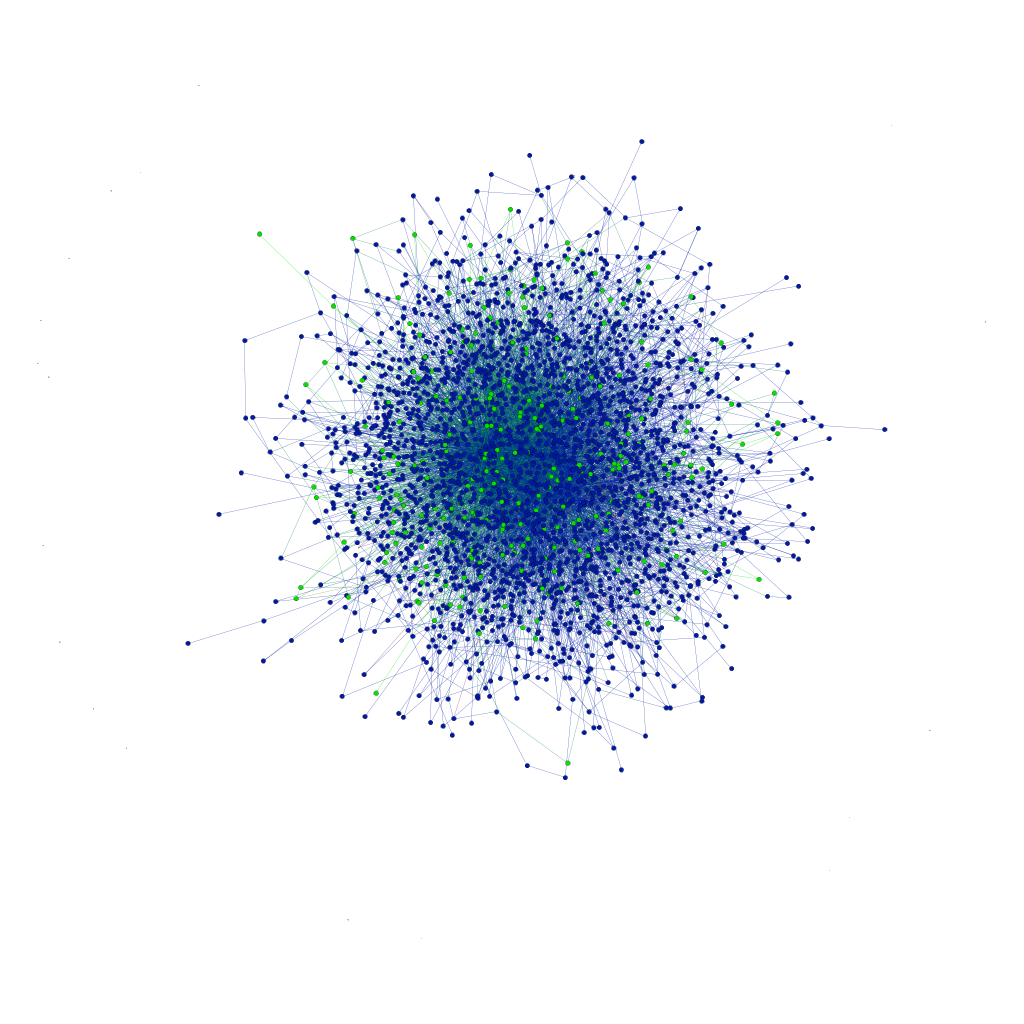
\includegraphics[scale=0.4]{sample-fin.png}
\end{center}
\caption{Sampled network at the end of the simulation. Note that lighter nodes are smokers, whereas darker ones are non-smokers.}
\label{img:sample-fin}
\end{figure}

More interestingly, if the smokers (figure \ref{img:email-nonsmok}) and non-smokers (figure \ref{img:email-smok}) are separated out into separate graphs, it can be seen that the remaining smokers at the end of the simulation are, mainly, highly connected. This explains the percentage of smokers remaining after such a large proportion of the graph was not smoking. They appeared to be influencing and supporting each other in continuing to avoid giving up. Finding this kind of group is very important in the attempt to encourage cessation as without direct intervention, their connectivity means the influence sways towards keeping smoking and nullifies those who attempt to persuade the nodes to give up. Having a cluster of non-smokers inside this group could break this influence and cause further cessation.

Furthermore, figure \ref{img:email-smok}, the separated non-smokers, appear to be of a form similar to a small-world network due to the large, central cluster. When compared to figure \ref{img:email-nonsmok}, the separated smokers, this is clear since the smokers appear to adopt a more scale-free form. The occurrence of the latter is revealed by a number of hub nodes which have a higher degree than average. To make a change within this sub-network of smokers, these hubs could be targeted since they have the potential to influence many other nodes and in turn, spread smoking cessation further. In terms of targeting groups for attempts to cause smoking cessation, it would seem that this type of network, similar to scale-free, is more effective than the non-smoker network, as in the latter higher connectivity means that many more nodes would have to be changed in order to spread the same behaviour. This is compounded by the fact that in small-world networks, hubs are much less prevalent and within a group of nodes, the chance of each being connected to another is high meaning that even highly influential nodes need the support of others to impart a certain behaviour.

\begin{figure}
\begin{center}
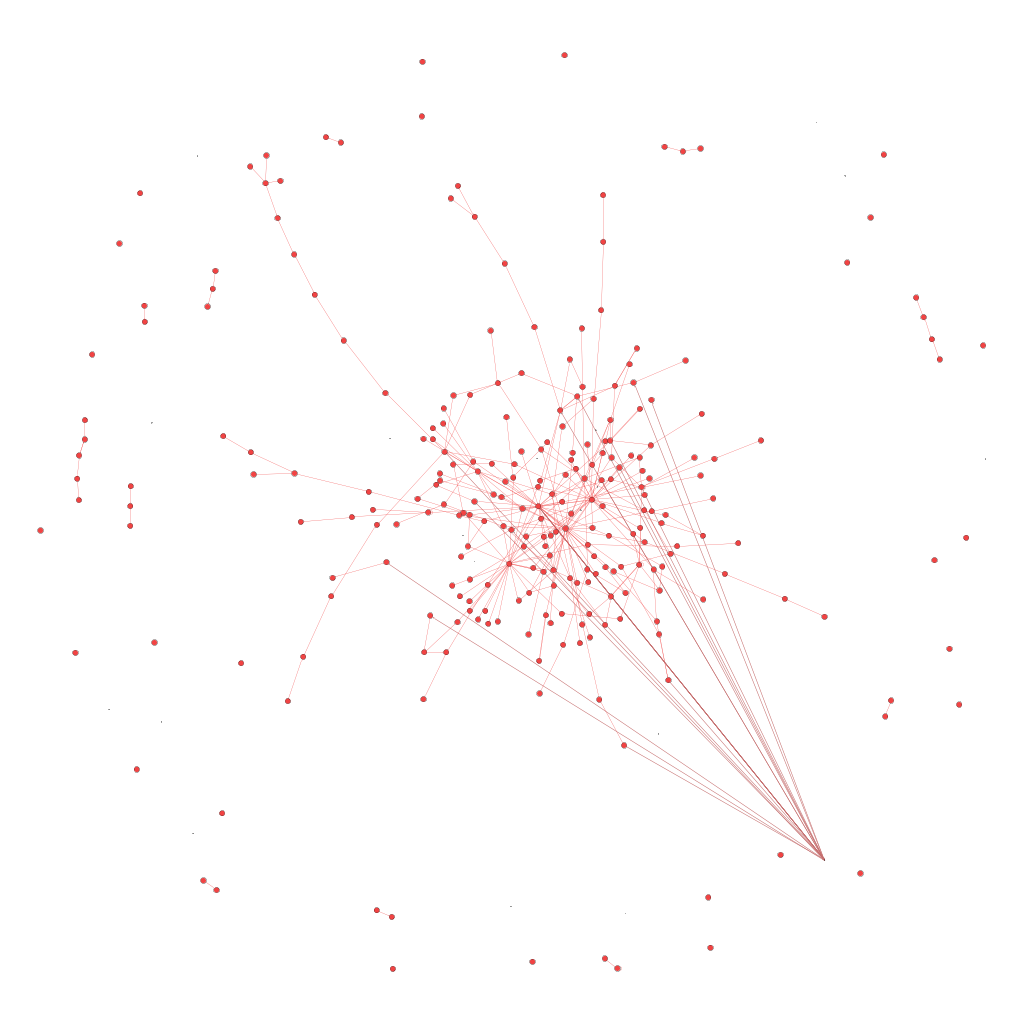
\includegraphics[scale=0.4]{email-smokers.png}
\end{center}
\caption{Smokers Within Email Dataset at 30,000 Steps - Note the scale-free type structure present between smokers at the end of the simulation, indicating why a core of smokers remained.}
\label{img:email-smok}
\end{figure}

\begin{figure}
\begin{center}
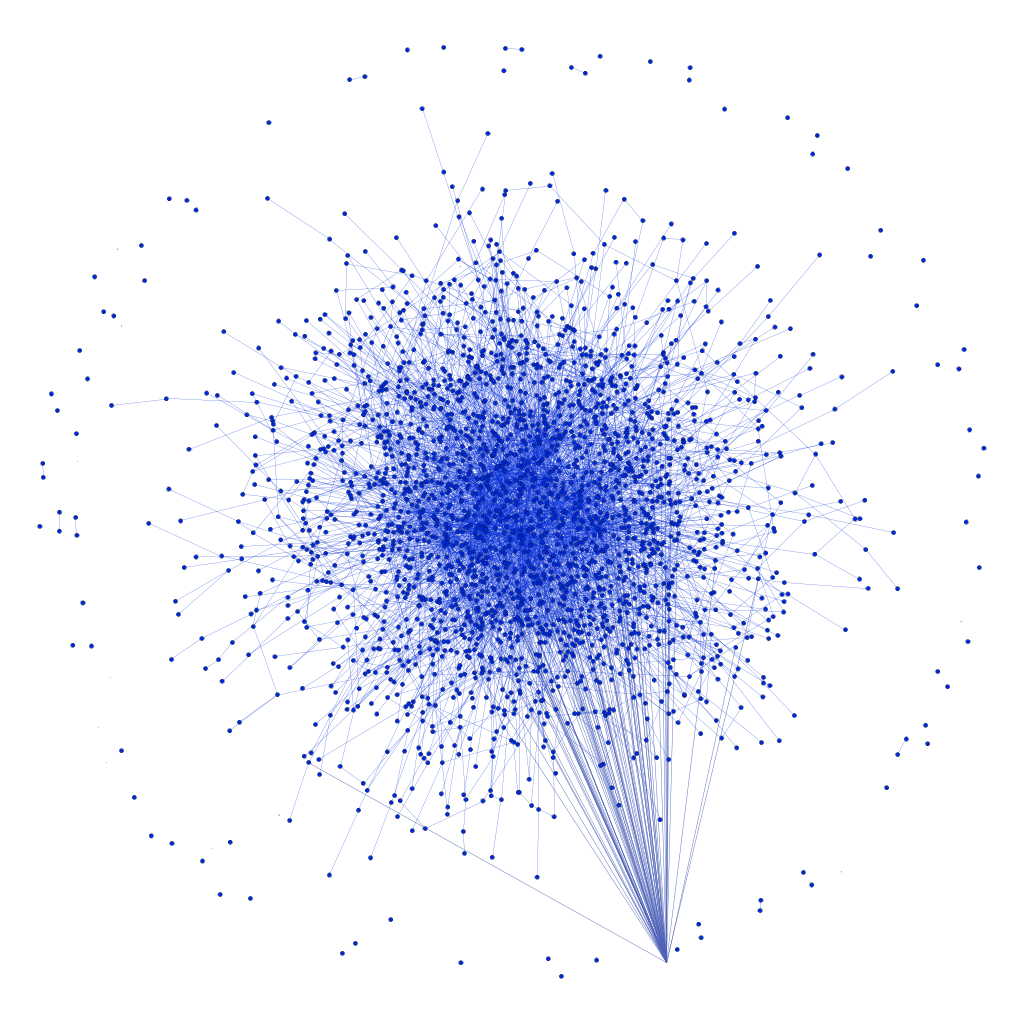
\includegraphics[scale=0.4]{email-nonsmok.png}
\end{center}
\caption{Non-Smokers Within Email Dataset at 30,000 Steps - A small-world type network is present, which explains the fact that most of the network are now non-smokers due to lots of influence about the non-smoking behaviour.}
\label{img:email-nonsmok}
\end{figure}

Using real-world datasets, as shown above, is useful when attempting to understand behaviours like smoking cessation but as can be seen in graphs such as figure \ref{img:sample-init}, the method of sampling lends itself to generating small-world type samples. As other sampling methods were not implemented, it cannot be ascertained that this structure is endemic of realistic graphs or the particular dataset, but the process of performing a derivative of a depth-first search means that some nodes are included which have extremely high degree as seen in figure \ref{img:email-smok}. These are the nodes that are used to start the sample or are reached in the early stages so whilst expected, it is not desirable since the nodes can take on a very influential role within the network. This does not detract from the results, however, as each node has the opportunity to have many other nodes influencing them which, due to the aggregate methods in calculating influence, reduce the impact of the hubs. As a final note, the type of network from which the data is sampled should be considered – some sampled networks may have more similarities with the type of network required by this project than others. This will have an effect on the results they produce, however understanding the requisite features for an ideal dataset is not part of this project.

\section{Commercial Viability \& Model Analysis}
\subsection{Commercial Viability Analysis}

Commercial viability analysis of this project mainly focuses on whether the current system could be used as a starting point in building a more in-depth model so looks at aspects such as:
\begin{itemize}
\item \emph{Efficient} - to save excess computing cycles on large and long-running simulations
\item \emph{Scalable} - to be able to run both small and very large models, allowing for analysis on a wide range of social situations such as small friendship groups to populations of cities or towns.
\item \emph{Extensible \& adaptable} - should new work influence the configuration of the model, it should not need entirely rebuilding in order to include these changes.
\end{itemize}

The efficiency of the model is good in places – the decision tree, for example, primarily uses \emph{if} statements for decisions with only basic arithmetic comparisons or pre-computed values rather than more complex values computed for each stage. Furthermore, the neighbourhood and influenced attributes are only calculated once per turn since these are both intensive operations and are used at many points within an agent turn.  Due to this system being a proof-of-concept, efficiency was not always the main concern during development with the favour instead being given to a functional and balanced model. This means that some inefficient sections are present, but are not so intertwined with other components in such a way that makes them difficult to fix.   

An example of this is related to the fact that the network structure can change from one agents turn to another; because of this, neighbourhoods have to be generated for every agent on every turn. This requires a lot of graph traversal and in larger graphs, a lot of processing time. Unfortunately, this was difficult as caching neighbourhoods introduces the chance of nodes who are newly removed from this set playing a role in calculations and verifying the neighbourhood requires the same amount of computation as creating it. One possible way to get around this is to cache the neighbourhood at the end of each agent turn. Changes could then be handled by, again at the end of each turn, having each agent broadcast its one-hop neighbours to its one-hop neighbourhood. These nodes can then check for the existence of neighbourhood nodes between the end of their turn and the start of the next – new ones can be added, whilst if they are unaccounted for then they can be removed.

Efficiency in the agent lends itself to scalability of the model in general. This is because the majority of the runtime is spent within agent actions so if these are made to be as efficient as possible the model will perform faster when more agents are added. Because this model is not developed with the intention of running simulations with in excess of 10,000 nodes not as much time has been spent on developing with the intention of running large scale tests though in a commercial solution, this would be very important. Developing in this manner requires attention to be split between individual agents and the system as a whole; for example, removing any actions carried out by every agent that could be done once for the whole network would save a lot of compute cycles. If performance was of paramount importance, then the stage at which network reconfiguration happens could be separated out from within the agent to for the whole network at once. This means that rather than agents would work on a fixed network each turn rather than one which changes between separate agent turns meaning steps such as scoring between agents would need to be carried out fewer times.

With regards to scalability, some more fundamental changes would need to be made in order to provide good performance on large systems. Agent-based systems are difficult to scale due to the amount of processing power required for even smaller ones as even in this project, a basic representation of humans and their connections require the performance of many different operations per step. As more agents are added, on top of the internal processing for this new addition, each existing agent may now have even more nodes in its neighbourhood, resulting in more calculations per agent. The exact effect of more agents being added can depend on a number of factors, such as its degree, size of neighbourhood and more making it difficult to quantify.

To better analyse this, simulations and graph generations were carried out on a variety of graph sizes on both generated small-world and scale-free graphs. Each simulation ran for 30,000 steps and was timed with the results being plotted. For reference, the tests were carried out on a 3.4GHz quad-core, Intel i5 processor, using 1.3GB of RAM for the Java Virtual Machine. Graph generation is a one-off step in a simulation that, in its most general sense, will create a graph of size $n$ agents each with a set of attributes and social connections. It should be noted that if a sampled graph is used, the time taken for $n$ nodes to be prepared for running will be less than that of a scale-free graph being generated since the sampled graph simply uses the attribute creation step that scale-free graphs also use without having to create the graph structure first. Because of this upper bound, tests were not carried out on them

\begin{figure}
\begin{center}
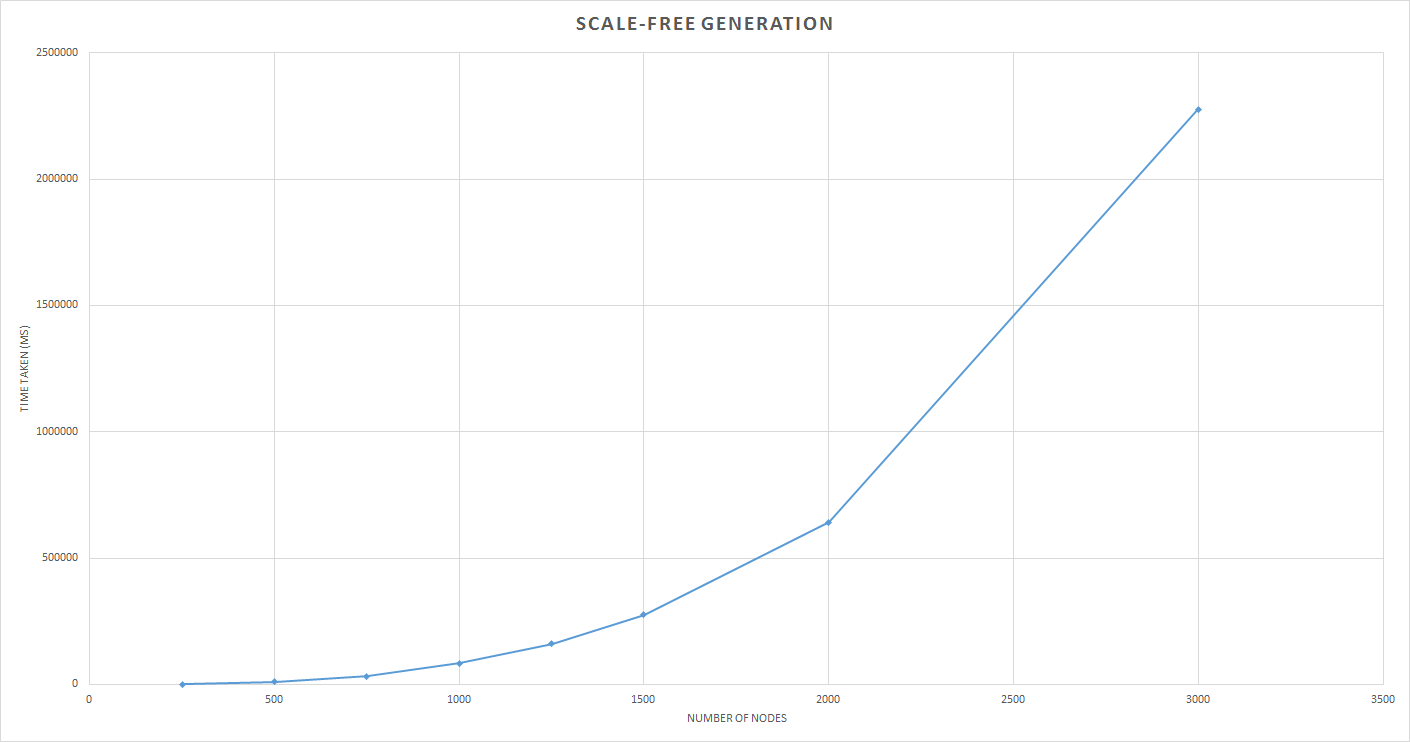
\includegraphics[width=\textwidth]{scale-free-gen.png}
\end{center}
\caption{Scale-Free Generation: Time taken (ms) against the size of graph generated where a lower time is more desirable. Note the almost quadratic increase as the number of nodes increases.}
\label{img:SF-gen}
\end{figure}

\begin{figure}
\begin{center}
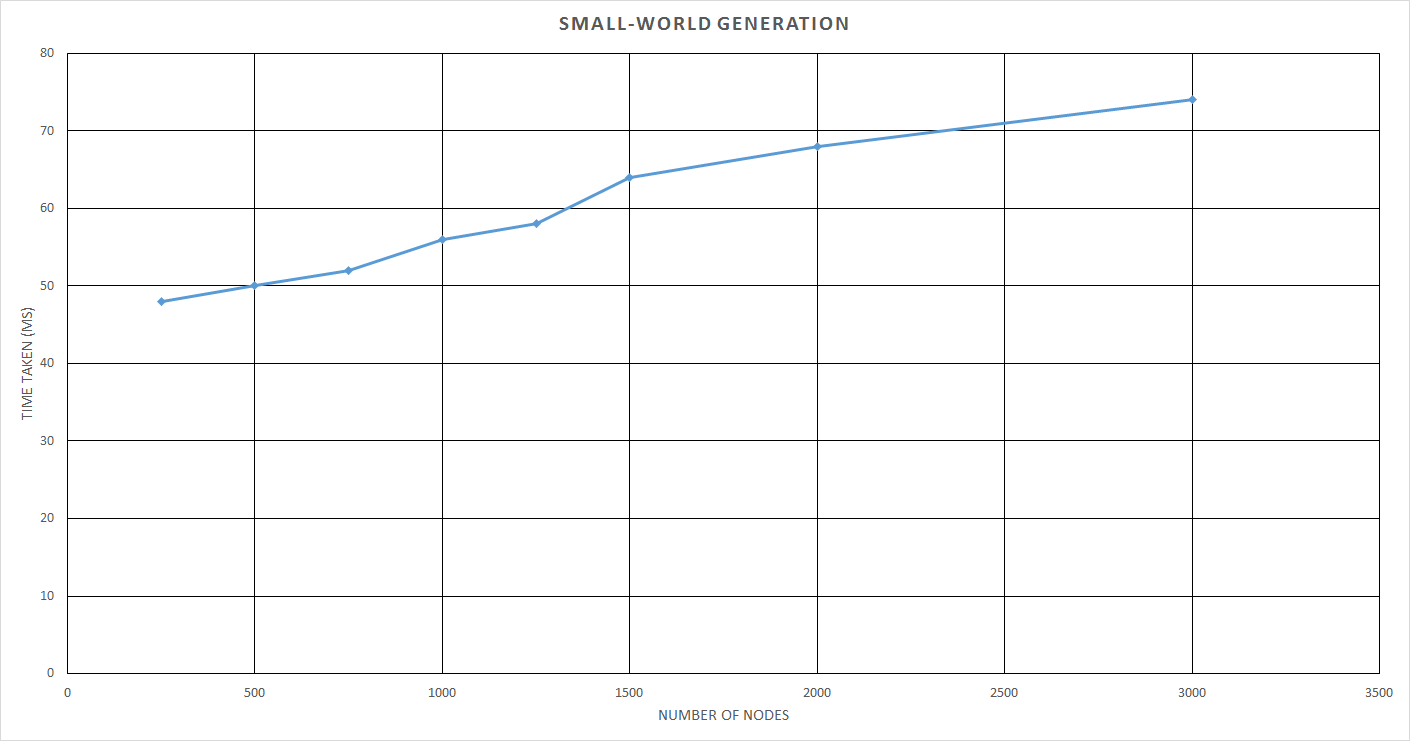
\includegraphics[width=\textwidth]{small-world-gen.png}
\end{center}
\caption{Small-World Generation: Time taken (ms) against the size of graph generated where a lower time is more desirable. A linear trend is shown as the number of nodes increases, whilst the overall time to generate is very low.}
\label{img:SW-gen}
\end{figure}

As visible in figure \ref{img:SF-gen}, the generation time for scale-free graphs increases in an almost quadratic fashion as the number of nodes increases, reaching around 30 minutes for a 3000 node graph. Adding to this, as the generation method leaves disconnected nodes in the graph which have to be removed causing the final node count to often be lower. Obviously, this level of performance would not be effective in a commercial environment since large graphs of over 1000 nodes would take too long to create. This, however, may be partly due to the implementation rather than the method; figure \ref{img:SW-gen} shows the generation times for a small-world graph using the \textbf{Repast} built-in small-world creation algorithm. A very short creation time across the range of node counts had a linear increase which is a better performance, however the method for generating small-world graphs is much less intensive than that of scale-free because of the incremental addition of nodes in the latter. This is in part also caused by the calculation used to determine if an edge is to be added or removed being simpler for small-world graphs than scale-free. From this, it can be seen that to make this aspect of the model more commercially viable, it needs to offer a more scalable generation method for scale-free graphs.

\begin{figure}
\begin{center}
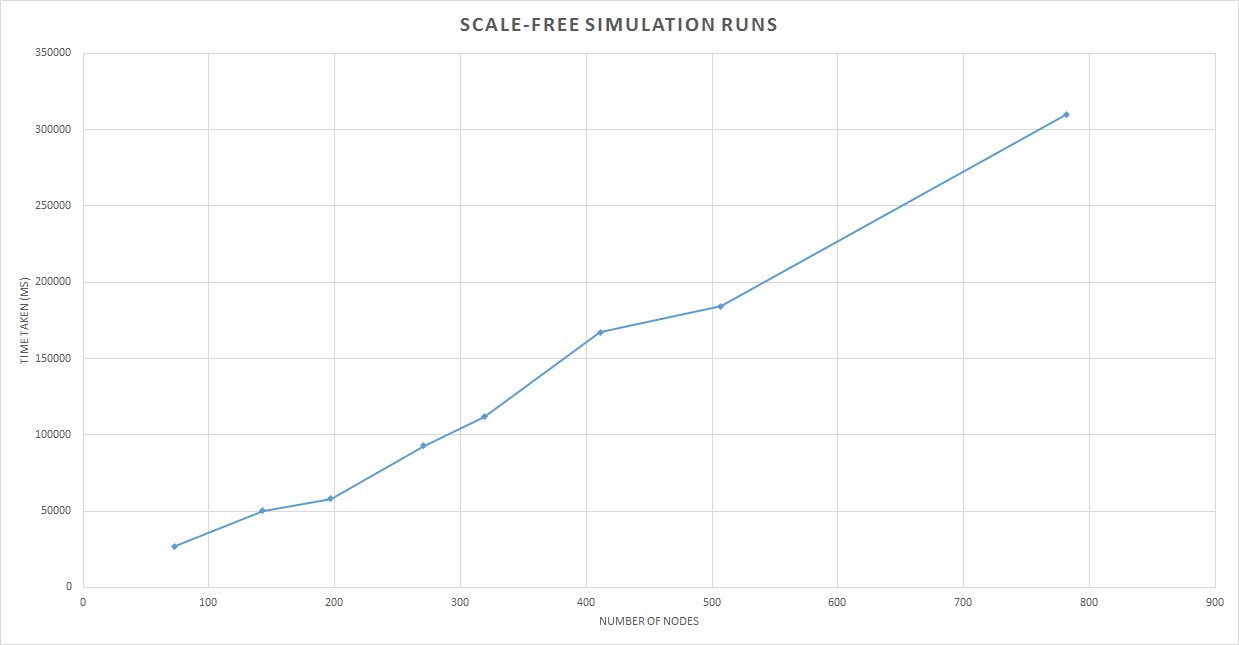
\includegraphics[width=\textwidth]{scale-free-runs.png}
\end{center}
\caption{Scale-Free Runs: Time taken (ms) against the size of graph generated where a lower time is more desirable. Although steep, as the number of nodes increase, the time taken for that run increases in a linear fashion.}
\label{img:SF-run}
\end{figure}

\begin{figure}
\begin{center}
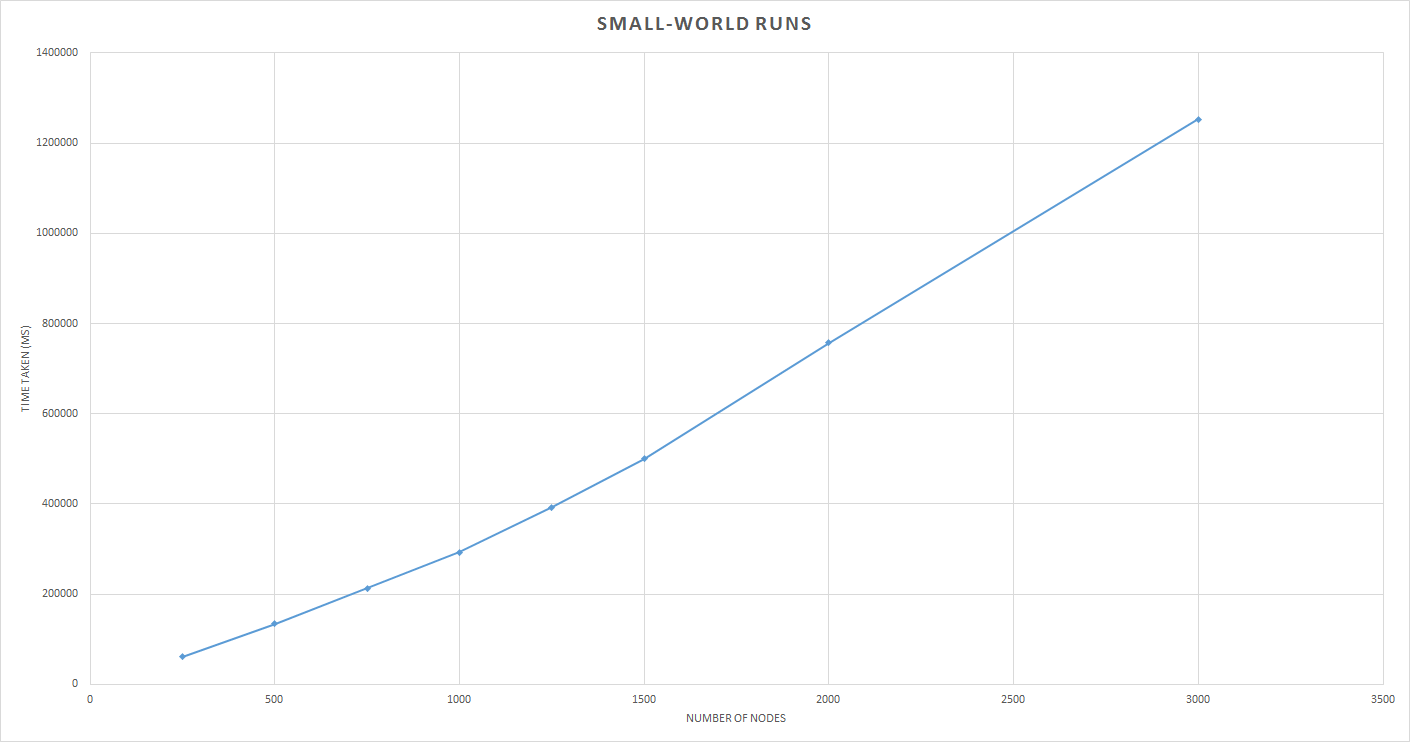
\includegraphics[width=\textwidth]{small-world-runs.png}
\end{center}
\caption{Small-World Runs: Time taken (ms) against the size of graph generated where a lower time is more desirable. As with small-world generation (figure \ref{img:SW-gen}), the time taken increases linearly with the number of nodes in the run.}
\label{img:SW-run}
\end{figure}

Perhaps more important than this is the time taken for simulations to run. This is a difficult area to quantify since two graphs of identical node count can vary in many ways such as edge density, average degree and more, in turn affecting how the graph may behave. Using the graphs generated for the previous tests, the results of the simulations carried out can be seen in figures \ref{img:SF-run} and \ref{img:SW-run}. A point to note is that due to the scale-free method not producing graphs of exactly the number of nodes required, creating a 3000 node graph to match the upper limit of the small-world tests would have been very difficult. It can be seen that both follow a roughly linear increase as nodes are added, with simulations of around 750 nodes taking around 4 minutes for a small-world graph and just over 5 minutes for a scale-free one. The similarity in the trends of these graphs indicate that the type of graph may be independent of how long a simulation on it takes. If this is the case for all graphs, then the focus for scalability improvements lie within agent efficiency, as detailed above. In regards to the simulation times with the current implementation, although 20 minutes for a 3000 node small-world graph may seem high, if run on a cluster or HPC, the runtime would be much shorter. As such, increasing the number of agents significantly would not cause untenable runtimes should the requisite computing power be available. From this basic investigation, the model appears to be fairly scalable but would benefit from work on agent efficiency if simulations were to take place on personal computers or to maximise compute cycles.

On the whole, the system displays a good level of extensibility and ease of maintenance. From the start of development, focus has been on building not only a useful model but also a platform on which it is easier to improve said model. This was done by ensuring that any tools developed were written in as general a manner as possible, as well as grouping them into related packages. The agent itself separates out its actions into methods, especially the three steps of neighbourhood finding, running the decision tree and reconfiguring connections. A useful feature that this allows is the easy replacement of any of these components, without having to disentangle them from the rest of the agent implementation - a company could use this to create a number of separate approaches to the decision tree and network reconfiguring and test them by simply changing the method calls.

Furthermore, the \emph{Repast} framework is a large, public project which causes it to be well-organised and ensures that user code is separated from system code. By making user code interface with the system instead of building within it, modifications to said system can be avoided and the efficiency and speed of the underlying simulator can be guaranteed. This is important since it shifts the emphasis for code to be well written and efficient. Furthermore, keeping this separation means that if the model implementation is maintainable, the developer does not need to worry about the simulation environment code. A side note is that the model is developed within \emph{Repast Simphony} whereas a commercial level model would probably require HPC access and due to this would need to be translated to C++ for \emph{Repast HPC}. Assuming the same principles would be used in translating the model as in creating it, this task would not need as much time or effort to develop and so would not be a major problem.

As a final note, whilst the original intention was to work with Sandtable, an agent-based modelling company, commercial pressures during the course of the project meant that they had less involvement than planned. Although this was the case, high-level reviews of both the social networking and decision making methods were undertaken with feedback being positive. The project success was not affected by this lack of involvement since a more general view of commercial needs was adopted.

\subsection{Model Analysis}
Overall, the model did provide insight into the problem domain and from this could be judged successful. Considering the fact that the intention was for the system to hold a proof-of-concept status and keeping the modelling of both the agent and network to basic levels, it is encouraging to see that the project does seem to exhibit behaviours that would be expected such as being able to run on networks without collapsing into tight clusters but at the same time with the network actually changing. Furthermore, as described above, it does produce results that indicate how networks can be manipulated in order to aid in causing smoking cessation. With this in mind, a number of other points that are important in the development of this type of model were discovered.

A major factor during the development of the project was that of balancing the model. Trial and error indicated that balance was indicated by how long the social network could avoid collapsing into tight clusters or becoming too sparse; for example, if a scale-free network collapses into a small-world network in fewer than 10,000 simulation steps then the model would appear to be very imbalanced, whilst a collapse over a longer period of time would indicate a better configuration and so would be more useful. It was found that certain aspects of the system had a much greater impact on this balance than others:
\begin{itemize}
\item \emph{Connection reconfiguration add/remove boundaries} - a lower bound of 0.4 and upper bound of 0.7 was used throughout simulations though whilst finding this boundary set, many others were tried. As might be expected, raising the lower bound too high caused the graph to become sparse over time, since it would be overzealous with edge removal. On the other hand, dropping the upper bound by just 0.05 caused the network become saturated with edges very quickly, resulting in many feedback loops and lots of edges becoming high influence.
\item \emph{Decision tree end-state inputs} - the values which are fed into the decisions that choose if a person starts or stops smoking significantly affects the distribution of smokers to non-smokers. Setting the thresholds too low makes it very easy for that decision to cause a change such as smoker to non-smoker, meaning that agents will readily make this change and move between two states regularly. In contrast, setting the values too high means that extraordinary situations are required for changes in behaviour which may never happen. This would cause very little change in the graph and could cause it to become stale, reaching a saddle-point very quickly.
\item \emph{Decision ordering} - the order in which an agent reaches decisions changes the significance of attributes since on average, the higher in the decision tree it is the more agents will encounter it. For example in the tree of this model, the most important decision is for whether the person is a smoker so it is at the top. If willpower was placed at the top of the tree instead, then any changes to willpower would have a much greater effect on agent behaviour.
\item \emph{Influenced attributes} - given that these are generated based on the autonomous behaviour of the agent to the point of calculation, there is a chance that influence causes these values to tend towards the extremities of their ranges. Should these attributes be used as the basis of decisions within the tree, this can cause entire branches to be inaccessible to agents, heavily skewing the balance of the tree and by extension, the model.
\end{itemize}
If the model were to be used for further research, these areas should be the focus when it comes to rebalancing.

Behaviour-wise, the model generally performs as expected but with some areas that could be improvemed. The fact that it can be configured to avoid mass clustering indicates that the interaction between agents can perform in a similar but basic manner compared to human behaviour. This appears to be done by maintaining a number connections that are of different influence levels with others whilst avoiding having a very high number of these connections - much like a person would find it difficult to maintain a lot of friendships simultaneously. Furthermore, the manner in which connections are reconfigured uses an abstract representation of evaluating likenesses meaning that similar people aim to connect with each other and, due to this connection, then influence each other. In social networking terminology, this is form of homophily, as described in the Literature Review (Section \ref{sec:litrev}). Given that this is observed in real-world networks, its occurrence here is useful.

An area in which some more unexpected behaviours occurred was that of attaining consistent results being difficult. Over a number of runs, the same simulation configuration can give a wide range of finishing splits between smokers and non-smokers which means that for results to be determined, many iterations must be run then averaged. Even if this is the case, if the spread of results is uniform across the range this would imply that the particular parameters used have little effect on the final state. This is hard to change because the model relies on agent autonomy and in doing so, variance between iterations should be expected; as such, a lack of consistency may be endemic due to using agent-based modelling. Accounting for this involves paying attention not only to the number of iterations used but also the variance and distribution of the results.

Some of the more specific undesirable behaviours, whilst minor, can have an impact on the model at large. Firstly, it appears that the model makes beginning smoking (and particularly relapsing) too easy, resulting in a number of give-up attempts over the course of the simulation or, in extreme cases, constant switching between being a smoker and non-smoker. This is not ideal as the spurious changes raise the number of attempts at giving up, possibly nullifying the impact of previous attempts. As a result, these agents do not provide a source of influence consistent with one behaviour. Another observation was that of there being few, if any, individuals giving up at the end of the simulation but instead are either smokers or non-smokers. As agents that do give up and then relapse increase their chances of relapsing in the future, repeating this failure a number of times will mean that any attempts to give up are likely to fail rapidly. Ultimately this is a model stability issue and to address it a better method of having willpower and previous attempts at giving up would need to be developed that could incorporate the time since the last effort, amongst other attributes. Doing this would also contribute towards solving the issue of it being too easy to begin smoking, especially for those who are at risk of relapsing.

From the results above, it is clear that the decision tree for cessation and social networking part of the model do have worth since they provide the opportunity for the manipulation agents whilst tracking these changes, allowing for analysis of particular model configurations. The decision tree provides a good way to keep the decision-making process simple whilst offering a range of different choices to the agents and because of how the values for said decisions can be changed, the balance of the tree can be adjusted with ease. The network itself proved to be a good representation of real-life networks, allowing the opportunity for both generated and sampled networks to be simulated upon. Influence within the model was built into the decision tree ensuring that the social influence did actually affect the choice of behaviours. This was further reinforced by the end-states in the tree relying on the behaviour of the neighbourhood; in retrospect, this weighs a little too heavily in favour of the actions of those around the agent so the inclusion of willpower or stubbornness would help to recreate those who will behave in a certain way regardless of their surroundings. Obviously, for a commercial level model, the tree would be greatly expanded with more attributes added to the agent; this would then give further configurability and more insight into the different areas of smoking cessation. Coupled with further integration of influenced attributes into the tree, the decision tree and graph approach is promising.

\subsection{Further Improvements}
Given that this model is a starting point rather than a complete solution to the problem, there are many possible changes that would bolster the performance and accuracy. These range from minor changes to reworking of entire sections and in general were not included due to time constraints or simply being too complex.

The agent itself could be adjusted to include more attributes and for those already included, more accurate modelling. The former is a difficult proposition since to make these additions, it should be the case that the attributes have been shown to have some effect on smoking through other research. Due to how circumstantial smoking behaviours seem to be, acquiring general information about factors in smoking cessation is not straightforward. To undertake this, the best route would be to undertake research in the field with the specific intention of understanding smoking behaviour contributing factors. In spite of this, some attributes such as stress could be included, assuming a reasonable model could be incorporated which would account for both internal and external contributors to the stress. Accurately modelling existing parameters is easier since as shown in the Research \& Literature Review (Section \ref{sec:litrev}), work towards this has already been done. The process for each attribute would involve isolating each concept and investigating it individually, through which a mathematical model could be developed for it. To prove the accuracy, these models would then have to be tested against some real-world measure. Whilst this would aid in the general result quality of the model, it could incur extra computational cost which may be a problem if large simulations are the main focus. Avoiding this would then require either efficient attribute representations or only modelling the most significant ones in such a detailed manner.

In terms of the decision tree, there are a number of design-level changes that, whilst would not impact the operation of the tree, would allow for much faster and easier tree prototyping, in turn making it more straightforward when developing new or adapting existing trees. A modular approach could be used where a decision is represented by some abstract type, allowing the specification of attributes to decide on and their thresholds as well as some list of which decisions lead to others. This would remove the need for extra programming when implementing new decision trees so would make the model more usable for those who do not know how to program. On top of this, it would be easier to build visualisation tools for and get an understanding of the tree at a glance compared to the current implementation which uses \emph{nested if} statements.

Another decision-tree based change would be the inclusion of `dead-zones', which are tree states that result in no change to behaviours and/or attributes. By defining more `no change' behaviours, this would provide another aspect of configurability and  produce more gradual results. An extension to this would be to separate out physical and mental attributes. This would allow for influence, for example, to act upon mental state which in turn acts upon the individuals decisions and physical behaviours. Combined with the idea of dead-zones, gradual changes could be made to the mental attributes resulting in more of a `decision-making over time' behaviour by the agent.

Finally, some extra tools would be very useful in order to produce graphs more accurate to real-world ones. Examples of this would be to generate graphs that could have configurable clusters such as groups of smokers, or of highly connected nodes. This would provide better emulation of smaller, dense social circles within a larger network, similar to groups of friends and their interactions with other groups. This would require elements of both small-world and scale-free graphs, so neither method alone would be suitable to generate them. Additionally, some method of specifying specific attribute changes within agents at certain points of the simulation would be very useful in investigating how changes within a subset of nodes affects the network at large. This could allow a network to be set up and run for an amount of time before some pre-determined changes happen, providing a more organic simulation compared to starting with the network changes required.


% --------------------------------
%
%			END OF RESULTS
%
% --------------------------------

% --------------------------------
%
%			  CONCLUSION
%
% --------------------------------
\chapter{Conclusion}

Producing an agent-based model had a number of challenges associated with it. Firstly and most significantly, attaining balance within the model was very difficult due to the amount of interaction and influence within the system. This lead to a lot of time being spent on adjusting this balance and trying to maintain it which in turn meant that the scope of the work had to be restricted. Whilst a model with many features and little balance could have been created, it would have provided no useful results as even at the most basic level, extracting a ‘baseline’ for the simulations would be extremely difficult. The scope restriction did result in slightly less depth to agent features such as the decision tree and network reconfiguration but by not implementing this extra complexity, further, more extensive, balancing work was also avoided.

Adding to this is the size of this kind of task. As stated in this report, the model only intended to be a basic representation of both social networking and smoking behaviours but still required a great deal of background research and development. Taking this kind of model to a commercial level would require either a long period of time for a solo-developer or, to reduce this timescale to a more reasonable one, a team of developers experienced in agent-based modelling. Even then, it is likely that they would encounter the same type of issues seen within the development of this project but on a much larger and more complex scale.

The model itself, due to its limited number of attributes and interaction methods, is heavily influenced based. Multiple decisions rely on what the neighbourhood of a node is doing which, although important for the social aspect of the project, may not be as heavy an actor in such decisions. Should it be the case that it is a major part of the decisions, the introduction of further attribute changes, interaction methods and decision routes would add a lot of depth to the model and could provide a more detailed representation of human behaviour – this may then provide richer results from simulations which would aid analysis.

A useful part of the development time was that of platform creation. This involved building a series of tools and preparing the development environment in such a way to allow for creation of the model without having to spend too much time writing `wrapper code' to handle input and output, for example. Though it does not necessarily contribute to the project producing a good model, it did encourage consistent software development throughout and helped to organise code into a more manageable structure. 

As can be seen, a number of discoveries have been made through the course of this project, ranging from key factors in specific areas of the model to the task as a whole. In general, the main aim was to produce a model for investigating the interplay between smoking cessation and social networking. As can be seen in both the Implementation (Section \ref{sec:dev}) and Results (Section \ref{sec:analysis}), this was achieved and although not as decisive as one might hope, interesting insights into this interaction of fields were gained. Furthermore, through the research, development and analysis for this project, a number of areas that would warrant further investigation have been highlighted. Given that the model is a proof-of-concept, the revealing of these areas opens up the possibility of further research and the development of a more comprehensive, commercial model of how smoking behaviours and social networking actions interact.
% --------------------------------
%
%			END OF CONCLUSION
%
% --------------------------------
\bibliographystyle{ieeetr}
\bibliography{biblio}
\end{document}